\documentclass[a4paper, english, 12pt, reqno, draft]{amsart}

% ---------------------------------------------------------------------------

% Usepackages recommended in mcom-l-template.tex if needed.

\usepackage{amssymb}
% \usepackage{graphicx}
% \usepackage[cmtip,all]{xy}

% ---------------------------------------------------------------------------

% Usepackages inserted by authors.

\usepackage[english]{babel}
\usepackage[utf8]{inputenc}
\usepackage{tikz,tikzscale}
\tikzset{>=latex}
\usepackage{xcolor}
\usepackage{enumerate}
\usepackage{booktabs,multirow}
\usepackage{amsfonts}
\usepackage{dsfont}
\usepackage[final]{listings}

%%%%%%%%%% Packages to help editing %%%%%%%%%%
\usepackage[notref,notcite]{showkeys} % Show labels.
\usepackage[mode=multiuser]{fixme} % Provide note, warning, error, fatal.
\FXRegisterAuthor{gk}{envgk}{GK}
\FXRegisterAuthor{ar}{envar}{AR}
\FXRegisterAuthor{ss}{envss}{SS}
\fxusetheme{color}

% ---------------------------------------------------------------------------

% Theorems in the AMS style.

\newtheorem{theorem}{Theorem}[section]
\newtheorem{lemma}[theorem]{Lemma}
\newtheorem{corollary}[theorem]{Corollary}

\theoremstyle{definition}
\newtheorem{definition}[theorem]{Definition}
\newtheorem{example}[theorem]{Example}
\newtheorem{exercise}[theorem]{Exercise}

\theoremstyle{remark}
\newtheorem{remark}[theorem]{Remark}

\numberwithin{equation}{section}

% ---------------------------------------------------------------------------

% Newcommands by the authors.

\newcommand{\hyperHDG}{{\fontfamily{pzc}\selectfont \texttt{Hy}\hspace{-1.5pt}perHDG }}

\newcommand{\graph}{\ensuremath{\mathcal G}}
\newcommand{\setEdge}{\ensuremath{\mathcal E}}
\newcommand{\setNode}{\ensuremath{\mathcal N}}
\newcommand{\setNodeDir}{\ensuremath{\setNode_\textup D}}
\newcommand{\setNodeNeu}{\ensuremath{\setNode_\textup N}}
\newcommand{\setNodeInt}{\ensuremath{\setNode_\textup I}}
\newcommand{\setNodeBar}{\ensuremath{\bar{\mathcal N}}}
\newcommand{\setNodeDirBar}{\ensuremath{\setNodeBar_\textup D}}
\newcommand{\setNodeNeuBar}{\ensuremath{\setNodeBar_\textup N}}
\newcommand{\setNodeIntBar}{\ensuremath{\setNodeBar_\textup I}}
\newcommand{\edge}{\ensuremath{E}}
\newcommand{\node}{\ensuremath{N}}

\newcommand{\Graph}{\ensuremath{\boldsymbol{\mathcal G}}}
\newcommand{\SetEdge}{\ensuremath{\boldsymbol{\mathcal E}}}
\newcommand{\SetNode}{\ensuremath{\boldsymbol{\mathcal N}}}
\newcommand{\SetNodeDir}{\ensuremath{\SetNode_\textup D}}
\newcommand{\SetNodeNeu}{\ensuremath{\SetNode_\textup N}}
\newcommand{\SetNodeInt}{\ensuremath{\SetNode_\textup I}}
\newcommand{\SetNodeBar}{\ensuremath{\bar{\boldsymbol{\mathcal N}}}}
\newcommand{\SetNodeDirBar}{\ensuremath{\SetNodeBar_\textup D}}
\newcommand{\SetNodeNeuBar}{\ensuremath{\SetNodeBar_\textup N}}
\newcommand{\SetNodeIntBar}{\ensuremath{\SetNodeBar_\textup I}}
\newcommand{\Edge}{{\ensuremath{\boldsymbol E}}}
\newcommand{\RefEdge}{{\ensuremath{\widehat{\boldsymbol e}}}}
\newcommand{\LocEdge}{{\ensuremath{\boldsymbol e}}}
\newcommand{\Node}{{\ensuremath{\boldsymbol N}}}

\newcommand{\locDim}{\ensuremath{\mathfrak d}}
\newcommand{\globDim}{\ensuremath{\mathfrak D}}

\newcommand{\Der}{\ensuremath{\textup d_\Edge}}
\newcommand{\Nabla}{\ensuremath{\nabla_\Edge}}
\newcommand{\Div}{\ensuremath{\Nabla\!\cdot\!}}
\newcommand{\tangent}{\ensuremath{{\boldsymbol T}}}
\newcommand{\Normal}{\ensuremath{\mathfrak n_\Edge}}
\newcommand{\NormalOuter}{\ensuremath{\mathfrak n^\perp_\Edge}}
\newcommand{\RefNormal}{\ensuremath{\mathfrak n_\RefEdge}}
\newcommand{\LocNormal}{\ensuremath{\mathfrak n_\LocEdge}}
\newcommand{\jump}[1]{{[\![ #1 ]\!]}}
\newcommand{\diffeo}{\ensuremath{\Phi}}
\newcommand{\tangentMapping}{\ensuremath{\Phi_{\tangent(x)}}}
\newcommand{\orthProj}{\ensuremath{\Pi_{\tangent(x)}}}
\newcommand{\der}{\ensuremath{\textup D}}
\newcommand{\funcDet}{\ensuremath{g}}
\newcommand{\matQ}{\ensuremath{Q}}
\newcommand{\matR}{\ensuremath{R}}
\newcommand{\basis}{\ensuremath{\mathcal B}}
\newcommand{\unity}{\ensuremath{\mathds 1}}

\newcommand{\IN}{\ensuremath{\mathbb N}}
\newcommand{\IR}{\ensuremath{\mathbb R}}

\newcommand{\skeletal}{\ensuremath{\Sigma}}
\newcommand{\skeletalSpace}{\ensuremath{M}}
\newcommand{\skeletalSpaceCont}{\ensuremath{\mathcal M}}
\newcommand{\discElementSpace}{\ensuremath{V}}
\newcommand{\polynomials}{\ensuremath{\mathcal P}}

\renewcommand{\vec}[1]{\ensuremath{\boldsymbol{#1}}}
\DeclareMathAlphabet{\mathbfsf}{\encodingdefault}{\sfdefault}{bx}{n}
\newcommand{\vecc}[1]{\ensuremath{\mathbfsf{#1}}}
\newcommand{\Nu}{\ensuremath{\vec \nu}}
\newcommand{\dx}{\ensuremath{\, \textup d x}}
\newcommand{\dy}{\ensuremath{\, \textup d y}}
\newcommand{\ds}{\ensuremath{\, \textup d \sigma}}
\newcommand{\localU}{\ensuremath{\mathcal U}}
\newcommand{\localQ}{\ensuremath{\vec{\mathcal Q}}}
\newcommand{\localV}{\ensuremath{\mathcal V}}
\newcommand{\localR}{\ensuremath{\vec{\mathcal R}}}
\newcommand{\range}{\ensuremath{\mathcal R}}

\newcommand{\code}[1]{\texttt{#1}}

\newcommand{\longDef}{\ensuremath{u}}
\newcommand{\crossDef}{\ensuremath{w}}
\newcommand{\torsion}{\ensuremath{\varphi}}
\newcommand{\force}{\ensuremath{q}}
\newcommand{\momentum}{\ensuremath{m}}
\newcommand{\crossSect}{\ensuremath{\mathcal A}}
\newcommand{\mass}{\ensuremath{\mathfrak m}}
\newcommand{\eigenval}{\ensuremath{\underline \lambda}}
\newcommand{\deltat}{\ensuremath{(\Delta t)}}
\newcommand{\D}{\ensuremath{\textup D}}

% ---------------------------------------------------------------------------

% Make paragraph heading being small capitals!

\makeatletter
\def\paragraph{\@startsection{paragraph}{4}%
  \z@\z@{-\fontdimen2\font}%
  {\normalfont\scshape}}
\makeatother

% ---------------------------------------------------------------------------

% Define style of listings!

\definecolor{mygreen}{rgb}{0,0.6,0}
\definecolor{mygray}{rgb}{0.5,0.5,0.5}
\definecolor{mymauve}{rgb}{0.58,0,0.82}
\lstset{ 
  backgroundcolor=\color{white},   % choose the background color; you must add \usepackage{color} or \usepackage{xcolor}; should come as last argument
  basicstyle=\tiny,                % the size of the fonts that are used for the code
  breakatwhitespace=false,         % sets if automatic breaks should only happen at whitespace
  breaklines=true,                 % sets automatic line breaking
  captionpos=b,                    % sets the caption-position to bottom
  commentstyle=\color{mygreen},    % comment style
  deletekeywords={...},            % if you want to delete keywords from the given language
  escapeinside={\%*}{*)},          % if you want to add LaTeX within your code
  extendedchars=true,              % lets you use non-ASCII characters; for 8-bits encodings only, does not work with UTF-8
%  firstnumber= ,                   % start line enumeration with line 1000
  frame=single,                    % adds a frame around the code
  keepspaces=true,                 % keeps spaces in text, useful for keeping indentation of code (possibly needs columns=flexible)
  keywordstyle=\color{blue},       % keyword style
  morekeywords={*,...},            % if you want to add more keywords to the set
  numbers=left,                    % where to put the line-numbers; possible values are (none, left, right)
  numbersep=5pt,                   % how far the line-numbers are from the code
  numberstyle=\tiny\color{mygray}, % the style that is used for the line-numbers
  rulecolor=\color{black},         % if not set, the frame-color may be changed on line-breaks within not-black text (e.g. comments (green here))
  showspaces=false,                % show spaces everywhere adding particular underscores; it overrides 'showstringspaces'
  showstringspaces=false,          % underline spaces within strings only
  showtabs=false,                  % show tabs within strings adding particular underscores
  stepnumber=2,                    % the step between two line-numbers. If it's 1, each line will be numbered
  stringstyle=\color{mymauve},     % string literal style
  tabsize=2,                       % sets default tabsize to 2 spaces
%  caption={\lstname}                   % show the filename of files included with \lstinputlisting; also try caption instead of title
}

% ---------------------------------------------------------------------------

% Usepackage hyperref is the last to be added!

\usepackage[colorlinks = true, linkcolor = blue, citecolor = blue, urlcolor = blue]{hyperref}

% ---------------------------------------------------------------------------

% Document head as described in the template.

\begin{document}

\title[\hyperHDG --- HDG on hypergraphs]{\hyperHDG --- Hybrid discontinuous Galerkin methods for PDEs on hypergraphs and self-intersecting surfaces} 

\author{Andreas Rupp}
\address{Interdisciplinary Center for Scientific Computing (IWR), Heidelberg University, Mathematikon, Im Neuenheimer Feld 205, 69120 Heidelberg, Germany}
% \curraddr{}
\email{andreas.rupp@fau.de, andreas.rupp@uni-heidelberg.de}
\thanks{This work is supported by the Deutsche Forschungsgemeinschaft (DFG, German Research Foundation) under Germany's Excellence Strategy EXC 2181/1 - 390900948 (the Heidelberg STRUCTURES Excellence Cluster).}

\author{Guido Kanschat}
\address{Interdisciplinary Center for Scientific Computing (IWR) and Mathematics Center Heidelberg (MATCH), Heidelberg University, Mathematikon, Im Neuenheimer Feld 205, 69120 Heidelberg, Germany}
% \curraddr{}
\email{kanschat@uni-heidelberg.de}
% \thanks{}

\subjclass[2010]{\textcolor{red}{TODO}}

\date{\today}

% \dedicatory{}

\begin{abstract}
 \textcolor{red}{\textsc{Todo!}} 
 \\[1ex] \noindent \textsc{Keywords.}
 \textcolor{red}{TODO!}
\end{abstract}
% 
\allowdisplaybreaks
\maketitle
% 

\begin{envarnote}{Editing!}
 Dear all,
 
 since we are quite many people, I have included the usepackage ``fixme''. It provides quite powerful tools for editing text. You can use a note, a warning, an error, or a fatal to indicate things in the text. Using the initials it can be tracked who set a comment. Analogously, it works for warnings, errors, and fatals. Thus, using the command \verb|\arnote{This is a note by Andreas Rupp}| creates a note at the margins, where the ar in arnote stands for Andreas Rupp. Moreover, \verb|\begin{envarnote}{Short description} ..... \end{envarnote}| \linebreak will create a short description at the margin and a long text (like this) within the standard text.
\end{envarnote}
% 
\section{Introduction}
% 
Simulating flow and transport phenomena on \emph{hypergraphs}, i.e. self-intersecting surfaces or lines (in three dimensions), offers a wide range of possible applications for which hybrid methods seem extremely promising numerical tools. Thus, for example, \cite{HedinPE2019} uses the hybrid high order method to do flow simulations in discrete fracture networks.
% 
% ---------------------------------------------------------------------
\section{Hypergraphs}\label{SEC:hypergraph}
% ---------------------------------------------------------------------
% 
\hyperHDG is a simulation software to perform numerical experiments on so called hypergraphs. To this end, it is useful to discuss the composition of hypergraphs in some detail. At first, every hypergraph is defined as topological hypergraph, cf. Section. \ref{SEC:hypergraph_topology}. Additionally, a hypergraph may be equipped with a geometry, as illuminated in Section \ref{SEC:hypergraph_geometry}. 
% 
\subsection{Topological aspects of hypergraphs}\label{SEC:hypergraph_topology}
% 
In the whole manuscript, we consider a \emph{hypergraph} $\graph = (\setNode,\setEdge)$ consisting of a finite set of \emph{hypernodes} $\setNode = \{\node_1, \node_2, \ldots \}$ and a finite set of \emph{hyperedges} $\setEdge = \{\edge_1, \edge_2, \ldots \}$. All hyperedges $\edge \in \setEdge$ can be interpreted as connecting several nodes and, thus, can be written as $\edge \subset \setNode$.

Thus, the topology of a hypergraph $\graph$ is a pair consisting of a set of hyperedges $\setEdge$ and a set of hypernodes $\setNode$. Each hyperedge $\edge \in \setEdge$ is connected to other hyperedges via the set of its adjacent hypernodes. Note that this is exactly the inverted interpretation as compared to the aforementioned definition of a hypergraph, where nodes are interpreted as connected via edges.

\paragraph{Cubic and simplicial hypergraphs, and local dimension $\locDim$}
% 
We will define partial differential equations (PDEs) on hypergraphs. To do so, it helps---but is not necessary---to have an adequate graphical representation of hyperedges. For example, one might try to represent all $\edge \in \setEdge$ as (relatively) open unit hypercubes of dimension $\locDim \in \IN$. A hypergraph, of which all hyperedges $\edge = \{ \node_1, \node_2, \ldots, \node_{2\locDim} \}$ consist of exactly $2\locDim$ hypernodes, allows for such a representation of all hyperedges. The hypernodes may then be interpreted as the \emph{faces} (not the vertices) of the hypercubes/hyperedges and the hypergraph is denoted \emph{cubic} of \emph{local dimension} $\locDim$. In this representation, also the hypernodes are supposed to be (relatively) open sets.

Analogously, a hypergraph of which all hyperedges consist of $\locDim+1$ hypernodes is called \emph{simplicial} of local dimension $\locDim$.

\paragraph{Cubic/simplicial (topological) embeddings of hypergraphs to global dimension $\globDim$}
% 
If one wants to represent the whole hypergraph at once (instead of only single hyperedges), an embedding to an $\globDim$ dimensional space is needed. To allow for an easy notation, we denote by $\Edge \in \SetEdge$ the representation of $\edge \in \setEdge$ as (relatively) open, but smoothly deformed hypercube/simplex, by $\Node \in \SetNode$ the representation of a hypernode $\node \in \setNode$ as (relatively) open (deformed) face, and set $\Graph = (\SetNode, \SetEdge)$. A cubic/simplicial hypergraph can be \emph{topologically embedded} into $\IR^\globDim$ if
% 
\begin{enumerate}
 \item there is a way to assemble all deformed hypercubes/simplices (representing the hyperedges) such that for two different hyperedges $\edge^+ \neq \edge^-$ and two hypernodes $\node^- \neq \node^+$, we have $\Edge^- \cap \Edge^+ = \emptyset$ and $\Node^- \cap \Node^+ = \emptyset$.
 \item in the aforementioned assembly for all $\node \in \setNode$ and $\edge \in \setEdge$: We have $\Node \cap \Edge \neq \emptyset$ if, and only if, $\node \in \edge$.
\end{enumerate}
% 
\paragraph{Examples for cubic hypergraphs}
% 
According to this definition, every graph is both a cubic and a simplicial hypergraph. An illustration which can be interpreted as several hypergraphs---all embedded to $\globDim = 3$---can be found in Figure \ref{FIG:hyG_topo}:
% 
\begin{itemize}
 \item Cubic or simplicial hypergraph of $\locDim = 1$ consisting of twelve hypernodes (vertices) and  twenty hyperedges (lines).
 \item Cubic hypergraph of $\locDim = 2$ consisting of twenty hypernodes (lines) and eleven hyperedges (squares).
 \item Cubic hypergraph of $\locDim = 3$ consisting of eleven hypernodes (squares) and two hyperedges (cubes).
\end{itemize}
% 
\begin{figure}[ht]
 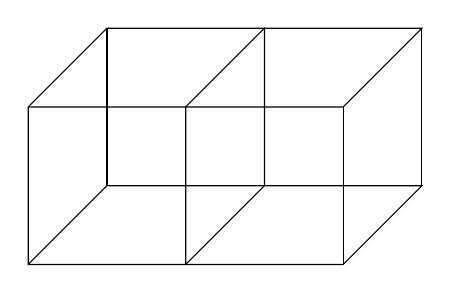
\begin{tikzpicture}
  \draw (0,0) -- (2,0) -- (4,0) -- (5,1) -- (3,1) -- (1,1) -- (0,0) -- (0,2) -- (2,2) -- (4,2) -- (5,3) -- (3,3) -- (1,3) -- (0,2);
  \draw (2,0) -- (3,1) -- (3,3) -- (2,2) -- (2,0);
  \draw (1,1) -- (1,3);
  \draw (4,0) -- (4,2);
  \draw (5,1) -- (5,3);
 \end{tikzpicture}
 \caption{Illustration that can be interpreted as several types of hypergraph topologies.}\label{FIG:hyG_topo}
\end{figure}
% 
\subsection{Geometrical aspects of hypergraphs}\label{SEC:hypergraph_geometry}
% 
Figure \ref{FIG:hyG_topo} already indicates that hypergraphs, especially those with embeddings might be equipped with geometrical information. This specific example indicates that all lines, squares, cubes are of unit size. However, the hypergraph might also have geometrical information that says it looks like in Figure \ref{FIG:hyG_geom}, where the first picture is valid for all $\locDim$ and the second one is only valid for $\locDim = 3$. Note that, all sufaces may also be curved, but we restrict to straight representations, here.
% 
\begin{figure}[ht]
 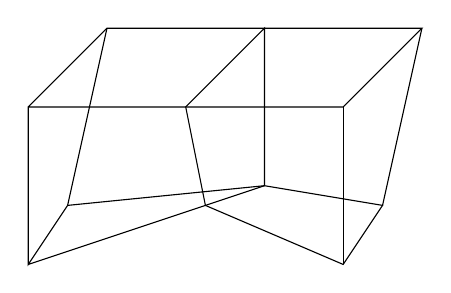
\begin{tikzpicture}
  \draw (0,0) -- (2.25,0.75) -- (4,0) -- (4.5,0.75) -- (3,1) -- (0.5,0.75) -- (0,0) -- (0,2) -- (2,2) -- (4,2) -- (5,3) -- (3,3) -- (1,3) -- (0,2);
  \draw (2.25,0.75) -- (3,1) -- (3,3) -- (2,2) -- (2.25,0.75);
  \draw (0.5,0.75) -- (1,3);
  \draw (4,0) -- (4,2);
  \draw (4.5,0.75) -- (5,3);
 \end{tikzpicture}
 \quad
  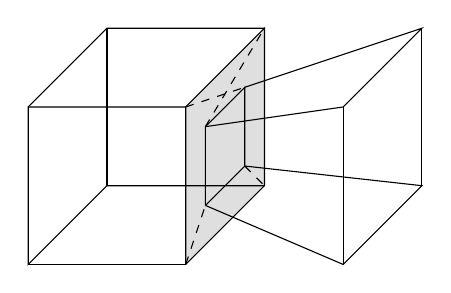
\begin{tikzpicture}
  \path[fill=gray!25] (2,0) -- (3,1) -- (3,3) -- (2,2) -- (2,0);
  \draw (0,0) -- (2,0);
  \draw[dashed] (2,0) -- (2.25,0.75);
  \draw (2.25,0.75)  -- (4,0) -- (5,1) -- (2.75,1.25);
  \draw[dashed] (2.75,1.25) -- (3,1);
  \draw (3,1) -- (1,1) -- (0,0) -- (0,2) -- (2,2);
  \draw (2.25,1.75) -- (4,2) -- (5,3) -- (2.75,2.25); 
  \draw (3,3) -- (1,3) -- (0,2);
  \draw[dashed] (2,2) -- (2.75,2.25);
  \draw[dashed] (2.25,1.75) -- (3,3);
  \draw (2,0) -- (3,1) -- (3,3) -- (2,2) -- (2,0);
  \draw (2.25,0.75) -- (2.75,1.25) -- (2.75,2.25) -- (2.25,1.75) -- (2.25,0.75);
  \draw (1,1) -- (1,3);
  \draw (4,0) -- (4,2);
  \draw (5,1) -- (5,3);
 \end{tikzpicture}
 \caption{Two possible geometrical representation of the hypergraph in Figure \ref{FIG:hyG_topo}. The second one is only valid for $\locDim = 3$---the gray hypernode has different geometrical representations for the two adjacent hyperedges.}\label{FIG:hyG_geom}
\end{figure}

This motivates the following observation: A hypergraph can, beyond its topological information, carry geometrical information. That is, for all hyperedges, there is a geometry prescribed.

This can lead to the case that for one hypernode, different geometries are prescribed as illustrated gray in the right picture of Figure \ref{FIG:hyG_geom}. The hypernode can also be distorted as illustrated by the dashed lines indicating that the two top vertices have to interchange when reinterpreting the node as face of the one or the other hyperedge. This could not be easily illustrated in the picture if the right version of the hypernode was not smaller than the left version. Thus, the hypernode would look as if no reinterpretation is necessary, although in fact, it is.

\paragraph{Embedded hypergraphs}
% 
If the hypergraph can be topologically embedded to dimension $\globDim$ and carries geometrical information for the hyperedges, such that for all hypernodes, there is a unique geometrical description---excluding that the hypernode is distorted or has different shapes for different hyperedges, then the hypergraph can be \emph{topological and geometrical embedded} (for short, just \emph{embedded}) into $\IR^\globDim$. For the representation of the embedded hypergraph, we also use the notation with the bold symbols.

\paragraph{Smoothness assumptions}
% 
We assume that each hyperedge $\IR^\globDim \supset \Edge \in \SetEdge$ allows for a $C^\infty$ diffeomorphism
% 
\begin{equation*}
 \diffeo_\Edge \colon \; \IR^\locDim \supset \RefEdge ~\mapsto~ \Edge \subset \IR^\globDim,
\end{equation*}
% 
where the reference element $\RefEdge$ is either a unit simplex of a unit hypercube.

Thus, the $\Edge\in \SetEdge$ are \emph{Riemannian manifolds}, i.e., they are real, smooth manifolds, and for all $x \in \Edge$, they are equipped with an inner product $(\cdot,\cdot)_{\tangent(x)}$ with respect to the \emph{tangent space} $\tangent(x)[\Edge] \subset \IR^\globDim$ of the manifold $\Edge$ evaluated at point $x$. If no confusion is possible, the expression $[\Edge]$ is dropped. We set the inner product as standard \emph{Euclidean scalar product}
% 
\begin{equation*}
 (a,b)_{\tangent(x)} := (a,b)_{\IR^\globDim} =: (a,b) \qquad \text{ for all } a,b \in \tangent(x) \text{ and } x \in \Edge
\end{equation*}
% 
and define $\| x \|^2 := (x,x)$ for $x \in \IR^\globDim$.

\paragraph{Linear hypergraphs}
% 
A cubic/simplicial hypergraph is called \emph{linear} if all hyperedges $\SetEdge \ni \Edge \subset \IR^\globDim$ can be represented as image of an affine-linear mapping of a (reference) unit hypercube/simplex $\RefEdge \subset \IR^\locDim$. This implies that all faces are straight and that the transformation matrix is square if, and only if, $\locDim = \globDim$.
% 
% ---------------------------------------------------------------------
\section{Elliptic model equation and interpretation}\label{SEC:model_eq}
% ---------------------------------------------------------------------
% 
Here, we formulate the standard diffusion equation in mixed form defined on a hypergraph $\graph$ that for the moment is assumed to allow an embedding $\Graph$. The differential operators will be rigorously defined in Section \ref{SEC:diff_op}. Thus, for all $\edge \in \setEdge$ we approximate solutions $(u, \vec q)$ of
% 
\begin{subequations}\label{EQ:diffusion_mixed}
\begin{align}
 \tfrac{1}{d} \vec q + \Nabla u & = 0 && \text{ in } \Edge,\label{EQ:primal_dual}\\
 \Div \vec q & = f && \text{ in } \Edge,\label{EQ:div_is_f}
\end{align}
% 
for given functions $d,f\colon \Edge \to \IR$, where $d \ge d_0 > 0$ is denoted diffusion coefficient and $f$ is denoted right-hand side. Here, $u$ may be considered as concentration and $\vec q$ as flux of a chemical species diffusing on the hypersurface $\Edge$. Thus, $u$ is supposed to have an unique representation with respect to all $\Node \in \SetNode$. This mimics the continuity assumption that is necessary to obtain a global $H^1$ solution and is assumed to hold for all scalar unknowns in the remainder of this manuscript. It can be more rigorously formulated as:

We assume that for all hypernodes $\Node \in \SetNode$ there is $u_\node$ such that
% 
\begin{equation}\label{EQ:cont_const}
 u_\node =  \gamma_0 ( u|_\Edge ) |_\Node \qquad \text{ for all } \edge \in \setEdge \text{ with } \node \in \edge,
\end{equation}
% 
where $\gamma_0: H^1(\Edge) \to H^{1/2}(\partial \Edge)$ is the trace operator.

Additionally, we assume that there is a non-empty set $\setNodeDir \subset \setNode$ of Dirichlet hypernodes, a possibly empty set $\setNodeNeu \subset \setNode\setminus \setNodeDir$ of Neumann hypernodes, and the remainder set $\setNodeInt = \setNode \setminus (\setNodeDir \cup \setNodeNeu)$ of interior hypernodes. The following ideas motivate three different types of closing conditions:
% 
\begin{itemize}
 \item On hypernodes of Dirichlet type, the value of function $u$ is prescribed by function $u_\text D$.
 \item On hypernodes of Neumann type, outflow of the whole system/hypergraph with rate $g_\textup N$ is prescribed. The outflow of chemical species with respect to a hyperedge is defined via $\vec q \cdot \Normal$. Here, $\Normal$ is the outward unit normal with respect to the hyperedge, cf. Section \ref{SEC:normals}. Thus the sum of outflows of all hyperedges adjacent to the Neumann node should be equal to $g_\textup N$.
 \item Interior hypernodes are Neumann hypernodes with $g_\textup N \equiv 0$ describing conservation of the chemical species.
\end{itemize}
% 
For PDEs on manifolds or the full space, the sum of outflows of all hyperedges adjacent to a hypernode consists of either one (at the boundary) or two summands and typically is represented by the notion of a \emph{jump} $\jump{\vec q}$, which can be generalized to
% 
\begin{equation*}
 \jump{\vec q}_\Node = \sum^{\edge \in \setEdge}_{\edge \ni \node} \vec q_\Edge \cdot \Normal \quad \text{ with } \quad \vec q_\Edge = \vec q|_\Edge,
\end{equation*}
% 
turning the vector function $\vec q$ to a scalar and being defined for all hyppernodes. The subscript $\Node$ will be dropped if no confusion is possible. Using this generalization, the closing conditions can be formulated into the following equations:
% 
\begin{align}
 u & = u_\textup D && \text{ on } \Node \in \SetNodeDir,\label{EQ:dir_cond}\\
 \jump{\vec q} & = g_\textup N && \text{ on } \Node \in \SetNodeNeu,\label{EQ:neu_cond}\\
 \jump{\vec q} & = 0 && \text{ on } \Node \in \SetNodeInt.\label{EQ:int_cond}
\end{align}
\end{subequations}
% 
Thus, \eqref{EQ:diffusion_mixed} is a direct generalization of the standard diffusion equation in the whole space---even with the same notation---if we manage to find proper direct generalizations of normals and differential operators.

\eqref{EQ:int_cond} is the analog to the assumption that $\vec q \in H^\textup{div}$ resulting in $u \in H^2$ (under appropriate regularity constraints). Moreover, \eqref{EQ:neu_cond} \& \eqref{EQ:int_cond} can be equivalently rewritten assuming that $g_\text N \equiv 0$ on all $\Node \in \SetNodeInt$. Thus, \eqref{EQ:neu_cond} \& \eqref{EQ:int_cond} will be formulated as
% 
\begin{equation}\label{EQ:Neumann_cond1}
 \jump{\vec q} ~=~ g_\textup N \qquad \text{ on } \Node \in \SetNode \setminus \SetNodeDir
\end{equation}
% 
in the remainder of this manuscript.
% 
\begin{envarerror}{This should be checked carefully!}
% 
One could also, more generally, reformulate \eqref{EQ:Neumann_cond1} to
% 
\begin{equation}
 \jump{\vec q} ~=~ g_\textup N \qquad \text{ on } \Node \in \SetNode \setminus \SetNodeDir^\dagger
\end{equation}
% 
with $\setNodeDir^\dagger \subset \setNode$ and $\# \setNodeDir^\dagger = \# \setNodeDir$. This naturally allows for Cauchy's (combination of Dirichlet and Neumann) boundary conditions without global existence and uniqueness issues.
% 
\end{envarerror}
% 
\subsection{The notion of normals}\label{SEC:normals}
% 
In the following, we will define different notions of normals with respect to a hyperedge $\Edge \in \SetEdge$. The simplest type of normal is the \emph{outer normal} $\NormalOuter \in \IR^\globDim$, which is defined via
% 
\begin{equation*}
 \|\NormalOuter(x)\| = 1 \qquad \text{ and } \qquad (\NormalOuter(x), v) = 0 \quad \text{ for all } v \in \tangent(x).
\end{equation*}
% 
The second condition can be abbreviated to $\NormalOuter(x) \perp \tangent(x)$. For each point $x \in \Edge$ there either exist no ($\locDim = \globDim$), two ($\locDim = \globDim - 1$) or infinitely many outer normals.

Additionally, for $x \in \partial \Edge$, we define the \emph{inner normal} $\Normal \in \IR^\globDim$ as unique, outward pointing vector with
%
\begin{equation}\label{EQ:inner_const}
 \| \Normal \| = 1, \qquad \Normal \in \tangent(x), \qquad \Normal \perp \tangent(x) [\partial \Edge]
\end{equation}

Considering the the reference element $\RefEdge \subset \IR^\locDim$, we define the \emph{reference normal} $\RefNormal \subset \IR^\locDim$ on its boundary as as the unit outward pointing normal of the reference edge. Furthermore assuming that $\der \diffeo_\Edge(x) = \matQ_\Edge \matR_\Edge$ is an $\matQ \matR$ decomposition (a specific normalized one will be used in Section \ref{SEC:HDG_loc_prob}), we define the \emph{local normal} $\LocNormal \in \IR^\locDim$ as outward unit normal of
% 
\begin{equation*}
 \LocEdge := \widehat \matR_\Edge \RefEdge,
\end{equation*}
% 
where $\widehat \matR_\Edge \in \IR^{\locDim,\locDim}$ is the upper left $\locDim \times \locDim$ block of $\matR_\Edge$ (containing the non-zero entries). Note that if $\widehat \LocNormal \in \IR^\globDim$ is the vector containing $\LocNormal(\hat x)$ and zeros below its entries, and $\hat x = \diffeo^{-1}_\Edge x \in \partial \RefEdge$, we have
% 
\begin{equation}\label{EQ:def_inner}
 \matQ^T_\Edge \Normal(x) = \widehat \LocNormal.
\end{equation}
% 
This equation actually is used to determine inner normals, since constructing an outward pointing vector sufficing \eqref{EQ:inner_const} is not a trivial task.
% 
\subsection{Differential operators on hyperedges}\label{SEC:diff_op}
% 
Consider the smooth function $f: \Edge \to \IR$. Its \emph{directional derivative} in $x \in \Edge$ and direction $v \in \tangent(x)$ is defined as
% 
\begin{equation}\label{EQ:direc_der}
 [\Der f(x)](v) ~:=~ \frac{\textup d}{\textup d \tau} (f \circ \gamma)(\tau)|_{\tau = 0}
\end{equation}
% 
for any smooth curve $\gamma: (-1,1) \to \Edge$ with $\gamma(0) = x$ and $\gamma'(0) = v$.

Accordingly, the \emph{derivative} is defined as
% 
\begin{equation*}
 \Der f(x) \colon \tangent(x) \to \IR, \qquad \text{ \eqref{EQ:direc_der} holds for all $v \in \tangent(x)$.}
\end{equation*}
% 
Thus, $\Der f(x) \in \tangent^\star(x)$ which is the dual space of $\tangent (x)$ and there is a well-defined mapping $\Der f \colon \Edge \to \tangent^\star(x)$. According to Riesz' representation theorem, there is a unique \emph{gradient} $\Nabla f \colon \Edge \to \tangent(x)$ with
% 
\begin{equation*}
 (\Nabla f(x), v) = [\Der f(x)](v) \qquad \forall x \in \Edge, \forall v \in \tangent(x).
\end{equation*}
% 
In terms of muscial isomorphisms, that is
% 
\begin{equation*}
 \Nabla f = (\Der f)^\sharp \qquad \text{ and } \qquad \Der f = (\Nabla f)^\flat.
\end{equation*}

The definition of the \emph{divergence} of a smooth vector function $\vec f \colon E \to \tangent(x)$ can be done using an orthonormal basis $\basis$ of $\tangent(x)$---which contains $\locDim$ elements---and setting
% 
\begin{equation*}
 \Div \vec f: \Edge \to \IR, \qquad [\Div \vec f](x) = \sum_{b \in \basis} [\Der (f, b)_{\tangent(x)} (x)](b).
\end{equation*}
% 
\begin{envarerror}{Needs to be checked and fully formulated! It just came to my mind.}
% 
\subsection{Existence and uniqueness of solutions}\label{SEC:ExUnique}
% 
In this brief section, we show that there is an unique function
% 
\begin{equation}
 \lambda \in \skeletalSpaceCont := \left\{ \mu \in L^2(\bigcup_{\Edge \in \SetEdge} \partial \Edge) \; \bigg| \; \mu |_{\partial \Edge} \in H^{1/2} (\partial \Edge) \text{ for all } \Edge \in \SetEdge \right\}
\end{equation}
% 
representing the restriction of $u$ to the hypernodes and unique functions $u \in L^2(\bigcup \Edge)$ and $\vec q \in H^{\operatorname{div}}(\bigcup \Edge)$ that suffice \eqref{EQ:diffusion_mixed} in the weak sense.

At first, we recognize that (assuming that we have some $\lambda \in \skeletalSpaceCont$ given) the problem to find $u|_\Edge \in L^2(\Edge)$ and $\vec q_\Edge \in H^{\operatorname{div}}(\Edge)$ such that
% 
\begin{subequations}\label{EQ:cont_lambda}
\begin{align}
 \int_\Edge u_\Edge (\nabla \cdot \vec \varphi) \dx - \int_\Edge \frac{1}{d} \vec q_\Edge \cdot \vec \varphi \dx & = \int_{\partial \Edge} \lambda (\vec \varphi \cdot \Normal) \ds && \forall \vec \varphi \in H^{\operatorname{div}}(\Edge) \\
 - \int_\Edge \vec q_\Edge \cdot \nabla \psi \dx + \int_{\partial \Edge} (\vec q_\Edge \cdot \Normal) \psi \ds & = 0 && \forall \psi \in H^1(\Edge)
\end{align}
\end{subequations}
% 
allows for an unique solution on all edges $\Edge \in \SetEdge$. Thus, there is a linear mapping $\lambda \mapsto (\localU \lambda, \localQ\lambda)$ which is induced by solving this problem.

Moroever, the same holds for the problem to find $u_\Edge \in L^2(\Edge)$ and $\vec q_\Edge \in H^{\operatorname{div}}(\Edge)$ such that
% 
\begin{subequations}
\begin{align}
 \int_\Edge u_\Edge (\nabla \cdot \vec \varphi) \dx - \int_\Edge \frac{1}{d} \vec q_\Edge \cdot \vec \varphi \dx & = 0 && \forall \vec \varphi \in H^{\operatorname{div}}(\Edge) \\
 - \int_\Edge \vec q_\Edge \cdot \nabla \psi \dx + \int_{\partial \Edge} (\vec q_\Edge \cdot \Normal) \psi \ds & = \int_\Edge f \psi \dx && \forall \psi \in H^1(\Edge)
\end{align}
\end{subequations}
% 
inducing the mapping $f \mapsto (\localU f, \localQ f)$.

Then, we can write the nodal conditions weakly as finding $\lambda \in \skeletalSpaceCont$ with $\lambda = u_\text D$ on Dirichlet nodes and
% 
\begin{equation}
 \sum_{\node \in \setNode} \sum_{\edge \ni \node}^{\edge \in \setEdge} \int_\Node [\localQ f + \localQ \lambda] \cdot \Normal \mu \ds = \sum_{\node \in \setNode} \int_\Node g_\text N \mu \ds
\end{equation}
% 
for all $\mu \in \skeletalSpaceCont$ with $\mu = 0$ in Dirichlet nodes. The term including $\localQ f$ goes to the right-hand side and by \eqref{EQ:cont_lambda}, the remaining left-hand side is rewritten edge by edge, to gain
% 
\begin{equation}
 - \sum_{\edge \in \setEdge} \int_\Edge d \localQ \lambda \cdot \localQ \mu \dx = \sum_{\node \in \setNode} \int_\Node g_\text N \mu \ds - \sum_{\node \in \setNode} \sum_{\edge \ni \node}^{\edge \in \setEdge} \int_\Node \localQ f \cdot \Normal \mu \ds.
\end{equation}
% 
Obviously, the right-hand side is a linear form and the left-hand side is a negative semi-definite bilinear form (if Dirichlet nodes have been assumed to be homogeneous, which is possible extending the right-hand side as in standard finite element theory by subtracting the Dirichlet data $u_\textup D \in \skeletalSpaceCont$). To use Lax--Milgram, we multiply both sides with $-1$ and use a Poincare inequality which can be shown exactly analogous to \cite[Satz 6.21]{Dobrowolski2010}.
% 
\end{envarerror}
% 
% ---------------------------------------------------------------------
\section{HDG method on hypergraphs}\label{SEC:hdg_graph}
% ---------------------------------------------------------------------
%
In this section, we discuss the HDG method applied to the diffusion equation on a hypergraph. Thus, we first formulate the method in Section \ref{SEC:HDG_form} and discuss implementation aspects of local problems (including transformation rules for the necessary integrals and differential operators) in Section \ref{SEC:HDG_loc_prob}. At last, we describe an efficient way of solving the global system of equations arising from the HDG discretization in Section \ref{SEC:glob_system}.
% 
\subsection{HDG formulation}\label{SEC:HDG_form}
% 
Let $p\ge 1$ and $\polynomials_p$ be the space of (multivariate)
polynomials of degree up to $p$. Then, we define the space of piecewise polynomials on the skeleton $\skeletal := \bigcup_{\Node \in \SetNode} \Node$ by
% 
\begin{gather}\label{EQ:skeletal_space}
 \skeletalSpace := \left\{ \lambda \in L^2(\skeletal) \;\middle|\;
 \begin{array}{r@{\,}c@{\,}ll}
  \lambda_{|\Node} &\in& \polynomials_p & \forall \Node \in \SetNode\\
  \lambda_{|\Node} &=& 0 & \forall \Node \in \SetNodeDir    
 \end{array}
 \right\}.
\end{gather}
% 
The HDG method involves a local solver on each mesh hyperedge $\Edge \in \SetEdge$, producing hyperedge-wise approximations $U_\Edge \in V_\Edge$ and and $\vec Q_\Edge \in \vec W_\Edge$ of the functions $u$ and $\vec q$ in equation \eqref{EQ:diffusion_mixed}, respectively. We choose $V_\Edge = \polynomials_p$. Then, choosing $\vec W_\Edge = \polynomials_p^d$ in a mixed formulation yields the so called hybridizable local discontinuous Galerkin (LDG-H) scheme. We will also use the concatenations of the spaces $V_\Edge$ and $\vec W_\Edge$, respectively, as a function space on $\Omega$, namely
%
\begin{gather}\label{EQ:dg_spaces}
 \begin{aligned}
  \discElementSpace &:=\bigl\{ v \in L^2(\Omega) & \big|\;v_{|\Edge} &\in V_\Edge, &\forall \Edge &\in \SetEdge \bigr\},\\
  \vec W &:=\bigl\{ \vec q \in L^2(\Omega;\mathbb R^d) & \big|\;\vec q_{|\Edge} &\in \vec W_\Edge, &\forall \Edge &\in \SetEdge \bigr\}.
 \end{aligned}
\end{gather}
% 
The HDG scheme for \eqref{EQ:diffusion_mixed} on a mesh $\Graph$
consists of the local solver and a global coupling equation. The local solver is defined hyperedge-wise by a weak formulation
of \eqref{EQ:diffusion_mixed} in the discrete spaces
$V_\Edge \times \vec W_\Edge$ and defining suitable numerical traces and fluxes. Namely, given $\lambda \in \skeletalSpace$ find $U_\Edge \in V_\Edge$ and $\vec Q_\Edge \in \vec W_\Edge$ , such that
% 
\begin{subequations}\label{EQ:hdg_scheme}
 \begin{align}
  \int_\Edge \frac{1}{d} \vec Q_\Edge \cdot \vec p \dx - \int_\Edge U_\Edge \Div \vec p \dx & = - \int_{\partial \Edge} \lambda \vec p \cdot \Normal \ds \label{EQ:hdg_primary}\\
  - \int_\Edge \vec Q_\Edge \cdot \Nabla v \dx  + \int_{\partial \Edge} ( \vec Q_\Edge \cdot \Normal + \tau  U_\Edge ) v \ds
  & = \tau \int_{\partial \Edge} \lambda v \ds \label{EQ:hdg_flux}
 \end{align}
\end{subequations}
% 
hold for all $v \in V_\Edge$, and all $\vec p \in \vec W_\Edge$, and for all $\Edge \in \SetEdge$. Here, $\tau > 0$ is the penalty coefficient. While the local solvers are implemented hyperedge by hyperedge, it is helpful for the analysis to combine them by concatenation. Thus, the local solvers define a mapping
% 
\begin{gather}
 \begin{split}
  \skeletalSpace & \to \discElementSpace \times \vec W\\
  \lambda &\mapsto (\localU \lambda, \localQ \lambda),
 \end{split}
\end{gather}
% 
where for each hyperedge $\Edge \in \SetEdge$ holds $\localU \lambda = U_\Edge$ and $\localQ \lambda = \vec Q_\Edge$. In the same way, we define operators $\localU u_\textup D$ and $ \localQ u_\textup D$, where in \eqref{EQ:hdg_scheme}, $\lambda$ is replaced by $u_\textup D$ on Dirichlet nodes, and by zero otherwise. Analogously, we set  $\localU f$ and $ \localQ f$ for
$f\in L^2(\bigcup_{\Edge \in \SetEdge} \Edge)$, where now the local solutions are defined by the system
% 
\begin{subequations}\label{EQ:hdg_f}
 \begin{align}
  \int_\Edge \frac{1}{d} \vec Q_\Edge \cdot \vec p \dx - \int_\Edge U_\Edge \Div \vec p \dx & = 0 \label{EQ:hdg_f_primary}\\
  - \int_\Edge \vec Q_\Edge \cdot \Nabla v \dx  + \int_{\partial \Edge} ( \vec Q_\Edge \cdot \Normal + \tau U_\Edge ) v \ds & =  \int_{\Edge} f v \dx\label{EQ:hdg_f_flux}
 \end{align}
\end{subequations}

Once $\lambda$ has been computed, the HDG approximation
to \eqref{EQ:diffusion_mixed} on $\Graph$ will be computed as\arnote{Maybe, we should just have two local solvers: one for $\lambda$ and one for data!}
% 
\begin{gather}\label{EQ:construct_unk}
  \begin{split}
    U &= \localU \lambda + \localU u_\textup D + \localU f\\
    \vec Q &= \localQ \lambda + \localQ u_\textup D + \localQ f
  \end{split}
\end{gather}

The global coupling condition is derived through a discontinuous
Galerkin version of mass balance and reads: Find
$\lambda \in \skeletalSpace$, such that for all
$ \mu \in \skeletalSpace$
% 
\begin{equation}
 \sum_{\edge \in \setEdge} \sum^{\node \in \setNode \setminus \setNodeDir}_{\node \in \edge} \int_\Node \left[ \vec Q \cdot \Normal + \tau (U - \lambda) \right] \mu \ds = \sum_{\node \in \setNode \setminus \setNodeDir} \int_\Node g_\textup N \mu \ds.\label{EQ:hdg_global}
\end{equation}
% 
\subsection{Implementation aspects of local problems}\label{SEC:HDG_loc_prob}
% 
Trying to implement local problems \eqref{EQ:hdg_scheme} or \eqref{EQ:hdg_f}, we need efficient ways to evaluate integrals with respect to hyperedges or hypernodes, and the differential operators of Section \ref{SEC:diff_op}. We start with an improved way of formulating integrals of the type
% 
\begin{equation}
 \int_\Edge f \ds = \int_\RefEdge \left[f \circ \diffeo^{-1}_\Edge\right] \underbrace{ \sqrt{\det[(\der\diffeo)^T \der \diffeo]} }_{ =: \funcDet }\dx,
\end{equation}
% 
where $\der$ denotes the standard total derivative and $\funcDet$ is the functional determinant. Thus, $g$ can be interpreted as generalization of the determinant of $\der\diffeo$, which in general is not a square matrix. However, via $\matQ\matR$ decomposition
% 
\begin{equation}\label{EQ:QR_decomp}
 \der\diffeo = \matQ_\Edge \matR_\Edge, \qquad \der\diffeo \in \IR^{\globDim,\locDim}, \, \matQ \in \IR^{\globDim,\globDim}, \, \matR \in \IR^{\globDim,\locDim},
\end{equation}
% 
where $\matQ_\Edge$ is an orthogonal (square) matrix with with $\det \matQ_\Edge = 1$ and $\matR$ is an upper triangular matrix with $(\matR_\Edge)_{i,i} \ge 0$ for all $i \ge 2$.  $(\matR_\Edge)_{1,1}$ should be non-negative if this is possible without violating the aforementioned conditions. Note that all enries $(\matR_\Edge)_{i,j} = 0$, for $i > \locDim$ or $j > \locDim$. Thus, we can equivalently calculate
% 
\begin{equation}\label{EQ:det_gen}
 \funcDet = \left| \det\der\diffeo \right|, \qquad \det\der\diffeo := \prod_{i=1}^\locDim (\matR_\Edge)_{i,i}.
\end{equation}
% 
Note that from this representation, we can also deduce whether $\diffeo$ preserves orientation, i.e., $(\matR_\Edge)_{1,1} \ge 0 \Leftrightarrow \det\der\diffeo \ge 0$, or changes orientation, i.e., $(\matR_\Edge) \ge 0$. Thus, we have that $\det$ from \eqref{EQ:det_gen} is a direct generalization of the standard determinant and gives the same value for square matrices. Thus, it carries the same notation. Analogous considerations allow to evaluate integrals with respect to hypernodes.

For the transformation of gradient and divergence, we will investigate the transformation of directional derivatives, first. The general formulas can then be constructed by combining the different directional derivatives, but are not used for implementation, where all directional derivatives are treated independently. We have that
% 
\begin{align*}
 [\der_\RefEdge (f \circ \diffeo) (\hat x)](\hat v) ~=~ & \frac{\textup d}{\textup d \tau} (f \circ \diffeo \circ \gamma) (\tau)|_{\tau = 0} \\
 ~=~ & [\der_{\diffeo \circ \gamma} f ((\diffeo\circ\gamma) (0))] \cdot [\der_{\gamma} \diffeo(\gamma (0))] \cdot \der_{\tau} \gamma(0)\\
 ~=~ & [\Der f (x)] \left( \der_{\hat v} \diffeo(\hat x) \right) ~=~[\Der f (x)] (v)
\end{align*}
% 
for $\gamma(0) = \hat x := \diffeo^{-1}_\Edge x$ and $\gamma'(0) = \hat v$ with $v = (\der_{\hat x} \diffeo_\edge(\hat x))\hat v$ (matrix--vector product), and the hat indicating that functions or operators live on the reference element. Here, also $\der_{\hat v} \diffeo(\hat x)$ is the directional derivative and $\cdot$ indicates just a product and that not application of a function is meant. This need not be the scalar product, here. Thus, we formally recover
% 
\begin{equation*}
 [\Der f (x)] (v) = [\der_\RefEdge (f \circ \diffeo) (\hat x)]([\der_{\hat x} \diffeo_\edge(\hat x)]^{-1} v).
\end{equation*}
% 
This is a generalization of the standard transformation formula for directional derivatives. However, the inverse is not well-defined, since the the derivative of $\diffeo$ cannot be assigned to a square matrix. Nonetheless, due to $v \in \range (\der_{\hat x} \diffeo_\edge(\hat x))$, it is well-defined in the sense of a mapping.

To gain an efficient implementation for the gradient and the divergence, we next define a local, orthonormal coordinate system on the tangent $\tangent(x)$ by using the first $\locDim$ column vectors of $\matQ$ from \eqref{EQ:QR_decomp}. This basis, for the sake of implementation, is also used as the basis for the divergence, as described in Section \ref{SEC:diff_op}: $\basis = \{b_1, \ldots, b_\locDim\}$. Thus, we can write
% 
\begin{align*}
 [\Der f (x)] (b_j) ~=~ & [\der_\RefEdge (f \circ \diffeo) (\hat x)]([\der_{\hat x} \diffeo_\edge(\hat x)]^{-1} b_j)\\
 ~=~ & [\der_\RefEdge (f \circ \diffeo) (\hat x)] (\matR^{-1}_\Edge \matQ^T_\Edge b_j)\\
 ~=~ & [\der_\RefEdge (f \circ \diffeo) (\hat x)] (r_j)
\end{align*}
% 
where $r_j$ is the $j$th column of $\matR_\Edge^{-1}$. Note that the whole right hand side of this equation can be formulated in $\locDim$ dimensions only, due to our bold choice of orthonormal systems. Using this idea, we can formulate gradient and divergence on an element with respect to the local coordinate system $\basis$, i.e., we set
% 
\begin{equation}
 \Nabla f(x) = \sum_{j=1}^\locDim b_j [\Der f (x)] (b_j) = \sum_{j=1}^\locDim b_j [\der_\RefEdge (f \circ \diffeo) (\hat x)] (r_j),
\end{equation}
% 
and treat the divergence analogously (without the $b_j$ after the sums).
% 
\subsection{Global system of equations}\label{SEC:glob_system}
% 
Equation \eqref{EQ:hdg_global} can, equivalently be rewritten to finding $\lambda \in \skeletalSpace$ such that
%
\begin{subequations}\label{EQ:forms_def}
\begin{equation}\label{EQ:forms_equal}
 \tilde a(\lambda, \mu) ~=~ \tilde b(\mu)
\end{equation}
% 
holds for all $\mu \in \skeletalSpace$ with
% 
\begin{align}
 \tilde a(\lambda, \mu) ~=~ & \sum_{\edge \in \setEdge} \sum^{\node \in \setNode \setminus \setNodeDir}_{\node \in \edge} \int_\Node \left[ \localQ \lambda \cdot \Normal + \tau (\localU \lambda - \lambda) \right] \mu \ds,\label{EQ:bil_def}\\
 \tilde b(\mu) ~=~ & \sum_{\node \in \setNode \setminus \setNodeDir}\int_\Node g_\textup N \mu \ds \label{EQ:lin_def}\\
 & - \sum_{\edge \in \setEdge} \sum^{\node \in \setNode \setminus \setNodeDir}_{\node \in \edge} \int_\Node \left[ (\localQ f + \localQ u_\textup D) \cdot \Normal + \tau (\localU f + \localU u_\textup D) \right] \mu \ds,\notag
\end{align}
\end{subequations}
% 
inducing the \emph{statically condensed global system of equations}
% 
\begin{equation*}
 \tilde{\vecc A} \vecc x = \tilde{\vecc b}, \quad \text{ where } \quad \tilde{\vecc A}_{ij} = \tilde a(\mu_j, \mu_i), \, \vecc x_i = \mu_i, \, \tilde{\vecc b}_i = \tilde b(\mu_i),
\end{equation*}
% 
where $(\mu_i)_i$ forms a basis of $\skeletalSpace$. According to \cite[Thm.\ 2.1 \& (2.11.a)]{CockburnGL2009}, the bilinear form $a$ can be rewritten to a form that obviously allows to conclude that $\tilde{\vecc A}$ is symmetric \emph{negative definite}. Hence, the conjugate gradient (CG) method can be applied to solve the linear system of equations.

The CG method uses matrix--vector products. For doing a single matrix--vector product $\tilde{\vecc A} \vecc x = \vecc y$, one needs to (assume that initially $\vecc y = \vecc 0$,) go through all hyperedges and per hyperedge:
% 
\begin{enumerate}
 \item Identify the adjacent hypernodes carrying information about $\lambda$, i.e. the global degrees of freedom---encoded in $\vecc x$.
 \item Use the gained information to solve local problem \eqref{EQ:hdg_scheme}.
 \item Calculated $\int_\Node \left[ \localQ \lambda \cdot \Normal + \tau (\localU \lambda - \lambda) \right] \mu_i$ based on the result of the local problem, where $i$ is the local index of the degree of freedom.
 \item Find global index associated to $i$ and add result to $\vecc y$.
\end{enumerate}

% \subsection{Restore positive definiteness of the induced system}
% 
Defining the positive definite statically condensed stiffness bilinear form $a$ and the linear form $b$ as
% 
\begin{subequations}
\begin{equation}\label{EQ:forms}
 a(\lambda, \mu) = - \tilde a(\lambda, \mu), \qquad b(\mu) = - \tilde b(\mu)
\end{equation}
% 
allows to equivalently rewrite \eqref{EQ:forms_def} as
% 
\begin{equation}\label{EQ:glob_system_new}
 a(\lambda, \mu) = b(\mu),
\end{equation}
\end{subequations}
% 
where $a$ is a positive definite discretization of the laplacian.

The positive definiteness of $a$ can be obtained by \cite[Thm.\ 2.1]{CockburnGL2009} stating that
% 
\begin{equation*}
 a(\lambda, \mu) = \sum_{\edge \in \setEdge} \left[ \int_\Edge \frac{1}{d} \localQ \lambda \; \localQ \mu \dx + \sum^{\node \in \setNode \setminus \setNodeDir}_{\node \in \edge} \int_\Node \tau (\localU \lambda - \lambda) (\localU \mu - \mu) \ds \right].
\end{equation*}
% 
\subsection{Elliptic convergence analysis}
% 
Obviously, the HDG method for elliptic diffusion problems is consistent with respect to the solution guaranteed in Section \ref{SEC:ExUnique}.
% 
\begin{envarnote}{Analysis ideas.}
 The rest might work similar to standard HDG, I do not really know and believe this is not urgent.
\end{envarnote}
% 
\subsection{Numerical convergence tests}\label{SEC:diff_conv_ell}
% 
\begin{table}[t]
 \begin{tabular}{cc|@{\,}lcc@{\,}lcc@{\,}lcc}
  \toprule
  \multicolumn{2}{c|@{\,}}{poly.~deg.}  && \multicolumn{2}{c}{1}  && \multicolumn{2}{c}{2}   && \multicolumn{2}{c}{3} \\
  \cmidrule{4-5} \cmidrule{7-8} \cmidrule{10-11}
  \multicolumn{2}{c|@{\,}}{mesh}    && err & eoc && err & eoc && err & eoc   \\
  \midrule
  \multirow{6}{*}{\rotatebox[origin=c]{90}{$\globDim = 1$}}
  & $i = 0$ && 6.80e-2 & --- && 8.20e-3 & --- && 8.04e-4 & ---  \\
  & $i = 1$ && 1.86e-2 & 1.9 && 1.14e-3 & 2.8 && 5.55e-5 & 3.9  \\
  & $i = 2$ && 4.92e-3 & 1.9 && 1.51e-4 & 2.9 && 3.63e-6 & 3.9  \\
  & $i = 3$ && 1.27e-3 & 2.0 && 1.94e-5 & 3.0 && 2.31e-7 & 4.0  \\
  & $i = 4$ && 3.22e-4 & 2.0 && 2.46e-6 & 3.0 && 1.46e-8 & 4.0  \\
  & $i = 5$ && 8.13e-5 & 2.0 && 3.09e-7 & 3.0 && 9.19e-10& 4.1  \\
  \midrule
  \multirow{6}{*}{\rotatebox[origin=c]{90}{$\globDim = 2$}}
  & $i = 0$ && 2.80e-2 & --- && 4.51e-3 & --- && 4.88e-4 & ---  \\
  & $i = 1$ && 1.10e-2 & 1.3 && 7.74e-4 & 2.5 && 4.07e-5 & 3.6  \\
  & $i = 2$ && 3.55e-3 & 1.6 && 1.18e-4 & 2.7 && 2.98e-6 & 3.8  \\
  & $i = 3$ && 1.02e-3 & 1.8 && 1.66e-5 & 2.8 && 2.03e-7 & 3.9  \\
  & $i = 4$ && 2.80e-4 & 1.9 && 2.21e-6 & 2.9 && 1.34e-8 & 3.9  \\
  & $i = 5$ && 7.39e-5 & 1.9 && 2.88e-7 & 2.9 && 8.65e-10 & 4.0  \\
  \bottomrule
 \end{tabular}\vspace{1ex}
 \caption{$L^2$ errors (err) and estimated orders of convergence (eoc) for elliptic example of diffusion on a unit square.}\label{TAB:diff_el_conv}
\end{table}
% 
Here, we consider the standard HDG approximation (no post-processing) and evaluate $L^2$ errors of the elliptic problem
% 
\begin{equation}
 - \nabla \cdot (d \nabla u) = f \text{ in } \Omega, \qquad u = u_\text D \text{ on } \partial \Omega,
\end{equation}
% 
where $d = \tfrac{2}{\pi}$ and $u = \sin(\tfrac{\pi}{2}x)$. The right hand side $f$ is chosen accordingly and $\Omega$ is supposed to be the $\globDim$ dimensional unit cube $[0,1]^\globDim$ which is uniformly subdivided into $2^{\globDim i}$ identical cubes in the $i$th refinement step. The penalty coefficient $\tau$ is set to be one, and the errors (err) and estimated orders of convergence (eoc) are depicted in Table \ref{TAB:diff_el_conv}. We recognize that the achieved orders of convergence perfectly fit to the expected ones which are $p + 1$.

\begin{table}[t]
 \begin{tabular}{c|@{\,}lcc@{\,}lcc@{\,}lcc}
  \toprule
  \multicolumn{1}{c|@{\,}}{dimension}  && \multicolumn{2}{c}{1}  && \multicolumn{2}{c}{2}   && \multicolumn{2}{c}{3} \\
  \cmidrule{3-4} \cmidrule{6-7} \cmidrule{9-10}
  \multicolumn{1}{c|@{\,}}{mesh}    && err & eoc && err & eoc && err & eoc   \\
  \midrule
  $i = 0$ && 8.24e-2 & --- && 5.81e-2 & --- && 2.38e-2 & ---  \\
  $i = 1$ && 1.66e-2 & 2.3 && 9.61e-3 & 2.6 && 3.20e-3 & 2.9  \\
  $i = 2$ && 3.60e-3 & 2.2 && 1.61e-3 & 2.6 && 4.16e-4 & 2.9  \\
  $i = 3$ && 8.28e-4 & 2.1 && 2.76e-4 & 2.5 && 5.31e-5 & 3.0  \\
  $i = 4$ && 1.97e-4 & 2.1 && 4.79e-5 & 2.5 && 6.71e-6 & 3.0  \\
  $i = 5$ && 4.82e-5 & 2.0 && 8.39e-6 & 2.5 && 8.43e-7 & 3.0  \\
  \bottomrule
 \end{tabular}\vspace{1ex}
 \caption{$L^2$ errors (err) and estimated orders of convergence (eoc) of linear approximation to the diffusion equation for hypergraph.}\label{TAB:diff_hg_el_conv}
\end{table}
% 
Next, we consider a convergence example on a real hypergraph. It is constructed to approximate
% 
\begin{equation}\label{EQ:hypergraph_example}
 - \Nabla \cdot (d \Nabla u) = f \text{ in } \Edge \in \SetEdge, \qquad u = u_\text D \text{ on } \Node \in \SetNodeDir,
\end{equation}
% 
where the Dirichlet nodes are those that are located on the boundary of $[0,1]^\globDim$ with $\globDim = 3$. All other nodes are supposed to be interior nodes. The local dimension $\locDim = 1, \ldots, 3$, solution $u = -x^2 - y^2 - z^2$, diffusion coefficient $d = 1$, and right-hand side $f = 2 \locDim$. Of course, polynomial degrees $\ge 2$ are supposed to exactly reproduce the given solution, which is true in our numerical experiments. Thus, we only plot the errors for $p = 1$.
% 
Interestingly, the $L^2$ errors converge although with refinement, also the computational domain increases for $\locDim = 1$ and $\locDim = 2$. However, the rate of convergence is deteriorated by $1$ if $\locDim = 1$, and $\tfrac{1}{2}$ if $\locDim = 2$. The optimal order is obtained for $\locDim = 3$. Here, the optimal order appears to be $3 = p + 2$ instead of the expected $2 = p + 1$.
\begin{envarerror}{To be verified!}
 This might be due to the fact that the solution is quadratic and due to some super-convergence properties of LDG-H. For IP-H (cf.\ Section \ref{SEC:other_solvers}), this superconvergence does not apply.
\end{envarerror}
%
% ---------------------------------------------------------------------
\section{Structure of \hyperHDG}
% ---------------------------------------------------------------------
% 
The software library \hyperHDG implements the hybrid discontinuous Galerkin method on hypergraphs. Therefore, \hyperHDG is divided into two parts: The implementation of an \code{HDGhyperGraph} and of a \code{LocalSolver}. The program then runs as a loop over all hyperedges for which the local problems are solved and the results are written into some appropriate data structure.
% 
\subsection{Implementation of the HDG hypergraph}
% 
An \code{HDG\-Hyper\-Graph} consists of five parts:
% 
\begin{enumerate}
 \item Its \code{Topology} which is implemented as an abstract container class of \code{Topology::hyEdge}s. Each hyperedge knows the indices of the hypernodes which are adjoint to the hyperedge. Therefore, the full topology of the hypergraph can be reconstructed using this class only.
 \item Its \code{Geometry} which is also implemented as an abstract container class of \code{Geometry::hyEdge}s. Each hyperedge comprises its geometrical information (usually using a \code{Mapping} from some sort of reference element to the physical element. These \code{Geometry::\-¸hyEdge}s also contain information about all kinds of normals, transformation rules, etc.
 \item Its \code{NodeDescriptor} which is also implemented as an abstract container class of \code{NodeDescriptor::hyEdge}s. These hyperedges contain indices for all of their hypernodes. These indices, however describe the properties of the respective hypernodes. For example, all interior nodes (in whatever sense) might have index 0, Dirichlet nodes might have index 1, and Neumann nodes might have index 2 \ldots.
 \item A \code{DataContainer} (for each hyperedge) which is also implemented as an abstract container class of some auxiliary data the local solvers might produce and/or need, but cannot be (easily) constructed from other data, and thus needs to be stored. Since its structure depends on the respective local solver, its entries need to be defined in the local solver classes. For the aforementioned elliptic problem, its entries are empty, while for the following parabolic problem it might contain information about $U$ and $\vec Q$ of the previous time step.
 \item Its \code{HyperNodeFactory}. This class is the interface of the hypergraph to the global vector of unknowns. Thus, it serves via mapping hypernodes to entries in the global vector of unknowns and vice versa.
\end{enumerate}
% 
Using this abstraction, we basically decouple the topology from the geometry. The advantages of this approach have been discussed in Section \ref{SEC:hypergraph}. Moreover, the hypergraph is decoupled from the structures that are needed for the description of the PDE (i.e.\ its boundary conditions). To this end, the notion of different types of nodes arises which is not present in the definition of hypergraphs in Section \ref{SEC:hypergraph} but useful for our purposes. Last, but not least we have a separate class that is responsible for the local--to--global and global--to--local communication with respect to degrees of freedom.

Since \code{Topology}, \code{Geometry}, and \code{NodeDescriptor} are abstract containers, we define the return value of an \code{HDGhyperGraph} as a \code{hyEdge} which contains the topological, geometrical, and nodal information of a hyperedge.
% 
\subsection{Local problem solvers}
% 
The \code{LocalSolver} receives all the local data, i.e. the \code{hyEdge} and the local degrees of freedom, and solves \eqref{EQ:hdg_scheme} and/or \eqref{EQ:hdg_f}. Afterwards, it uses the local solution to provide the local contribution to the overall problem (which is then appropriately recombined by the global loops). Thus, the local solvers' implementations carry all information with respect to the partial differential equation and the HDG scheme. This includes the mapping of a node descriptor value to the type of node and the right-hand side function, etc. Typically, the local solvers return the local contributions to a matrix--vector product evaluation ($\vecc x \mapsto \vecc A \vecc x$), residual evaluation ($\vecc x \mapsto \vecc A \vecc x - \vecc b$), some error ($L^2$, \ldots), or they evaluate $U$ or $\vec Q$ for plotting.
% 
\subsection{Loops over all hyperedges}
% 
Global loops basically do the mapping of global degrees of freedom which are handed over to the local solver. Afterwards, they use the local solver's results and generate a global result---such as a global error number or global vector. Hence, the implementation of a loop over all hyperedges cares about the specific properties of the local solvers and the problem type. For that reason, there is one prototypical loop class for each PDE type. That is, we implemented global loops for (linear) elliptic problems, and one for each of the problem types that are discussed in Section \ref{SEC:related_diffusion_problems}. That is,
% 
\begin{itemize}
 \item one class for elliptic problems, cf. Section \ref{SEC:hdg_graph},
 \item one class for parabolic problems, cf. Section \ref{SEC:parabolic_diff},
 \item one class for the nonlinear eigenvalue approach, cf. Section \ref{SEC:diff_eigen},
 \item one class for the shifted inverse approach, cf. Section \ref{SEC:diff_eigen},
 \item and one loop class for the mass matrix approximation and its application to eigenvalue problems as discussed in Section \ref{SEC:approx_mass}.
 \item Additionally, we need a loop class for the solution of parabolic problems using an approximated mass matrix. However, this example is purely academical and not conducted in full detail.
\end{itemize}
%
These loop classes can then also be used for related problems like the Bilaplacian, cf.\ Section \ref{SEC:bilaplacian}, or elastic graphs, cf. Section \ref{SEC:elastic_beam}. Additionally, the plotting function technically is a global loop which does not refer to a specific problem type, but rather can be used by (almost) all problem types.
% 
% ---------------------------------------------------------------------
\section{Usage of \hyperHDG}
% ---------------------------------------------------------------------
%
"Using" \hyperHDG can be conducted in several steps: The first step consists in the ability to actually run and configure a problem that has been implemented in \hyperHDG in C++ or Python. Afterwards, we will describe the implementation requirements for local solvers and global loops such that new equations can be implemented. At last, we will briefly illuminate the implementation of hypergraphs.

In any case, it is important to read the README of \hyperHDG (especially the setup and installation guide) prior to using it. Installation of \hyperHDG is not explained in this manuscript.
%
\subsection{Using \hyperHDG via Python}
%
Using \hyperHDG in a Python script can be done by exploiting the script \code{cython\_import}. This way is discussed for the aforementioned elliptic diffusion problem by an example application. The script can be found in \hyperHDG's file \code{examples/\-diffusion\_elliptic.py}.

We start with importing the print function, and the packages \code{numpy}, \code{os}, \code{sys}, and \code{scipy}'s linear algebra tools. These packages will be used in the remainder of the Python script.
%
\lstinputlisting[language=Python, firstline=1, lastline=3, firstnumber=1]{../examples/diffusion_elliptic.py}
%
Next, we define some basic parameters such as the polynomial degree of both, the (discontinuous) polynomials which live on the skeletal, and the polynomials which are utilized by the local solvers, the dimension of a hyperedge $\locDim$, the dimension of the surrounding space $\globDim$, the refinement level of the domain, and whether we want the C++ code to be compiled in debug or release mode.
%
\lstinputlisting[language=Python, firstline=5, lastline=9, firstnumber=5]{../examples/diffusion_elliptic.py}
%
We have not used \hyperHDG so far. This will be changed in the next lines which try to import the interface \code{cython\_import}. If this is not successful, we add the path to \code{cython\_import}'s directory, which is the main directory of the repository, manually. Thus, the expression \code{os.path.dirname( os.path.abspath( \_\_file\_\_ ) ) + "/.."} might be changed to the path of \hyperHDG in self-written scripts.
%
\lstinputlisting[language=Python, firstline=11, lastline=15, firstnumber=11]{../examples/diffusion_elliptic.py}
%
Having imported \hyperHDG, we want to configure the possible problem, \hyperHDG should deal with. That is why, we create a \code{hyperhdg\_\-constructor} and set its properties to define our problem. Our problem is a standard elliptic problem, for which an elliptic global loop can be used. To inform ourselves about the features of an elliptic loop and those of possible other loops, the \code{doxygen} pages may be used. Our problem will be defined on a $\globDim$ dimensional (refined) unit cube's $\locDim$ dimensional elements. Thus, we need a cubic topology, a cubic node--descriptor, and the geometry of a unit cube. Moreover, the local solver to be chosen is our diffusion solver. Again, the meaning of the respective template arguments can be found in the \code{doxygen}. Here, \code{poly\_degree} refers to the order of the polynomial space, \code{2 * poly\_degree} refers to the order of the quadrature rule, the next parameter refers to a \code{struct} in which the utilized parameters (such as right-hand side, diffusivity, \ldots) are defined, and \code{double} is the used floating point arithmetic of the local solvers. The file in which the parameters \code{struct} is defined needs to be known to \hyperHDG. Thus, it is added to a list of (additional) include files. The other files are automatically found by \code{cython\_import}. The cython replacements define the constructor arguments (also denoted \code{constructor\_values} in the \code{doxygen}) of the topology and the geometry, and the debug mode is also transmitted to \code{cython\_import}.
%
\lstinputlisting[language=Python, firstline=17, lastline=25, firstnumber=17]{../examples/diffusion_elliptic.py}
%
With the statical configuration (the one that is needed for compilation of the C++ files) done, we can now define the class \code{hyperHDG} and create an element of this class by using its constructor. Note that it automatically fills the constructors for geometry and local solver with appropriate values. Nonetheless, the constructor might also comprise upto three elements. In this case, two vectors and an positive number (which represents the penalty in the LDG-H method). 
%
\lstinputlisting[language=Python, firstline=27, lastline=28, firstnumber=27]{../examples/diffusion_elliptic.py}
%
Now, we can start dealing with the actual problem. To do so, we create the global right hand side by evaluating the residual of $\vecc A \vecc x - \vecc b$ for $\vecc x = \vecc 0$ and multiplying the result by $-1$.
%
\lstinputlisting[language=Python, firstline=30, lastline=30, firstnumber=30]{../examples/diffusion_elliptic.py}
%
The matrix $\vecc A$ will not be calculated by \hyperHDG. Instead, the operator $\vecc x \mapsto \vecc A \vecc x$ is realized in a matrix-free fashion. Python's \code{scipy} package provides solvers for matrix-free situations. These solver require the definition of a \code{LinearOperator}, which is done in two lines:
%
\lstinputlisting[language=Python, firstline=32, lastline=33, firstnumber=32]{../examples/diffusion_elliptic.py}
%
Solving the linear system of equations can then be done using the CG method in one line. The remaining lines check that the CG method has converged.
%
\lstinputlisting[language=Python, firstline=35, lastline=38, firstnumber=38]{../examples/diffusion_elliptic.py}
%
In the case that the analytical solution is known, we can also evaluate the error and print it using:
%
\lstinputlisting[language=Python, firstline=40, lastline=40, firstnumber=40]{../examples/diffusion_elliptic.py}
%
Additionally, we can plot the calculated solution after setting some plot options whose meaning can be found in the \code{doxygen}.\begin{envarwarning}{To be adapted in code and tex!}However, this needs that a directory denoted \code{output} exists. If this is not the case, the directory, but not the actual output is created and the script needs to be rerun.\end{envarwarning}
%
\lstinputlisting[language=Python, firstline=42, lastline=45, firstnumber=45]{../examples/diffusion_elliptic.py}
%
\subsection{Using \hyperHDG via C++}
%
Alternatively, one can use \hyperHDG as C++ library. Please note that for this purpose, the \code{include} directory of \hyperHDG as well as the \code{include} directories of the submodules need to be added to the compiler's include paths. The flag \code{-DNDEBUG} compiles in release mode, while the code is created in debug mode if the flag is missing. Moreover, \hyperHDG needs to be linked to LAPACK, compiled with a standard of C++17, and the compiler needs to be able to find the parameters file in this example. Please check that your compiler meets the standards of \hyperHDG. Compilers that are tested against in pushes to the master branch and therefore should be safe can be found in the \code{Makefile}.

The code of the C++ program that does exactly the same as the aforementioned Python script can be found in the file \code{examples/\-diffusion\_elliptic.cxx}.

Since for C++, we do not have \code{cython\_import} that finds all the necessary files, we need to include them by hand. Since, we want to conduct the same example again, we have to include the geometry and the topology of a unit cube, as well as the elliptic global loop and the diffusion solver. Additionally, we need a sparse linear algebra providing the CG solver. Last, but not least the parameters need to be included.
%
\lstinputlisting[language=C++, firstline=1, lastline=6, firstnumber=1]{../examples/diffusion_elliptic.cxx}
%
This has prepared us to define the \code{main} function which will surround the rest of the code
%
\lstinputlisting[language=C++, firstline=8, lastline=9, firstnumber=8]{../examples/diffusion_elliptic.cxx}
%
and starts with defining the very same parameters as before.
%
\lstinputlisting[language=C++, firstline=10, lastline=13, firstnumber=10]{../examples/diffusion_elliptic.cxx}
%
Next, we define the problem class, where the different components have exactly the same meaning as in the \code{hyperhdg\_\-constructor} of the Python script. The only difference consists in the fact that this class can immediately be instantiated, which has not been the case in Python, where \code{cython\_import} had to build it first.
%
\lstinputlisting[language=C++, firstline=15, lastline=20, firstnumber=15]{../examples/diffusion_elliptic.cxx}
%
The remainder of the program also works analogously to the Python script, i.e., we first define the right-hand side as negative, homogeneous residuum,
%
\lstinputlisting[language=C++, firstline=22, lastline=24, firstnumber=22]{../examples/diffusion_elliptic.cxx}
%
solve the global system of equations using the CG method,
%
\lstinputlisting[language=C++, firstline=26, lastline=26, firstnumber=26]{../examples/diffusion_elliptic.cxx}
%
and print the $L^2$ error.
%
\lstinputlisting[language=C++, firstline=28, lastline=28, firstnumber=28]{../examples/diffusion_elliptic.cxx}
%
At the end, we plot the solution
%
\lstinputlisting[language=C++, firstline=30, lastline=33, firstnumber=30]{../examples/diffusion_elliptic.cxx}
%
and end the program returning 0.
%
\lstinputlisting[language=C++, firstline=35, lastline=36, firstnumber=35]{../examples/diffusion_elliptic.cxx}
%
\subsection{Writing global loops}
%
\textcolor{red}{TODO}\arnote{TODO!}
%
% ---------------------------------------------------------------------
\section{Related diffusion problems and approaches}\label{SEC:related_diffusion_problems}
% ---------------------------------------------------------------------
% 
\subsection{Post-processing and mixed approximation orders}\label{SEC:postprocess}
%
\begin{table}[t]
 \begin{tabular}{cc|@{\,}lcc@{\,}lcc@{\,}lcc}
  \toprule
  \multicolumn{2}{c|@{\,}}{poly.~deg.}  && \multicolumn{2}{c}{1}  && \multicolumn{2}{c}{2}   && \multicolumn{2}{c}{3} \\
  \cmidrule{4-5} \cmidrule{7-8} \cmidrule{10-11}
  \multicolumn{2}{c|@{\,}}{mesh}    && err & eoc && err & eoc && err & eoc   \\
  \midrule
  \multirow{6}{*}{\rotatebox[origin=c]{90}{$\globDim = 1$}}
  & $i = 0$ && 3.90e-2 & --- && 259e-3 & --- && 1.77e-4 & ---  \\
  & $i = 1$ && 5.18e-3 & 2.9 && 167e-4 & 4.0 && 5.64e-6 & 5.0  \\
  & $i = 2$ && 6.66e-4 & 3.0 && 1.06e-5 & 4.0 && 1.77e-7 & 5.0  \\
  & $i = 3$ && 8.44e-5 & 3.0 && 6.64e-7 & 4.0 && 5.53e-9 & 5.0  \\
  & $i = 4$ && 1.06e-5 & 3.0 && 4.15e-8 & 4.0 && 1.72e-10 & 5.0  \\
  & $i = 5$ && 1.33e-6 & 3.0 && 2.60e-9 & 4.0 && 5.40e-12 & 5.0  \\
  \midrule
  \multirow{6}{*}{\rotatebox[origin=c]{90}{$\globDim = 2$}}
  & $i = 0$ && 2.57e-2 & --- && 2.87e-3 & --- && 189e-4 & ---  \\
  & $i = 1$ && 4.82e-3 & 2.4 && 1.97e-4 & 3.9 && 6.55e-6 & 4.9  \\
  & $i = 2$ && 7.14e-4 & 2.8 && 1.31e-5 & 3.9 && 2.12e-7 & 4.9  \\
  & $i = 3$ && 1.01e-4 & 2.8 && 8.48e-7 & 4.0 && 6.82e-9 & 5.0  \\
  & $i = 4$ && 1.41e-5 & 2.8 && 5.46e-8 & 4.0 && 2.19e-10 & 5.0  \\
  & $i = 5$ && 1.97e-6 & 2.8 && 3.56e-9 & 3.9 && 7.14e-12 & 4.9  \\
  \bottomrule
 \end{tabular}\vspace{1ex}
 \caption{$L^2$ errors (err) and estimated orders of convergence (eoc) for elliptic example of diffusion on a unit square.}\label{TAB:diff_elpp_conv}
\end{table}
%
\begin{table}[t]
 \begin{tabular}{c|@{\,}lcc@{\,}lcc@{\,}lcc}
  \toprule
  \multicolumn{1}{c|@{\,}}{dimension}  && \multicolumn{2}{c}{1}  && \multicolumn{2}{c}{2}   && \multicolumn{2}{c}{3} \\
  \cmidrule{3-4} \cmidrule{6-7} \cmidrule{9-10}
  \multicolumn{1}{c|@{\,}}{mesh}    && err & eoc && err & eoc && err & eoc   \\
  \midrule
  $i = 0$ && 9.03e-2 & --- && 6.90e-2 & --- && 3.01e-2 & ---  \\
  $i = 1$ && 1.82e-2 & 2.3 && 1.13e-2 & 2.6 && 4.05e-3 & 2.9  \\
  $i = 2$ && 3.95e-3 & 2.2 && 1.90e-3 & 2.6 && 5.27e-4 & 2.9  \\
  $i = 3$ && 9.07e-4 & 2.1 && 3.26e-4 & 2.5 && 6.72e-5 & 3.0  \\
  $i = 4$ && 2.16e-4 & 2.1 && 5.67e-5 & 2.5 && 8.48e-6 & 3.0  \\
  $i = 5$ && 5.28e-5 & 2.0 && 9.92e-6 & 2.5 && 1.06e-6 & 3.0  \\
  \bottomrule
 \end{tabular}\vspace{1ex}
 \caption{$L^2$ errors (err) and estimated orders of convergence (eoc) of linear approximation to the diffusion equation for hypergraph.}\label{TAB:diff_hg_elpp_conv}
\end{table}

It is well known, both that the order of convergence of the LDG-H method can be increased by one using a local post-processing step and that the flux variable can be projected into $H^{\operatorname{div}}(\Omega)$ (by a Raviart--Thomas projection) without deterioration of convergence using a second local post-processing step. For further details on this topic, the reader may consult \cite{CockburnDGRS2009}.

The first post-processing (better convergence) can be conducted constructing $U^\star \in \polynomials_{p+1}(\Edge)$ $\forall \Edge \in \Graph$ from $U$ and $\vec Q$ such that for all $\Edge \in \Graph$
%
\begin{subequations}
\begin{align}
 \int_\Edge d \nabla U^\star \cdot \nabla v \dx & = - \int_\Edge \vec Q \cdot \nabla v \dx && \forall v \in \polynomials_{p+1}(\Edge),\\
 \int_\Edge U^\star \dx & = \int_\Edge U \dx
\end{align}
\end{subequations}
%
hold. Due to the super-convergence of the local means and the optimal $L^2$ convergence of $\vec Q$, $U^\star$ is supposed to $L^2$ converge with an order of $p+2$. This can also be seen from Tables \ref{TAB:diff_elpp_conv} \& \ref{TAB:diff_hg_elpp_conv} for the numerical examples of Section \ref{SEC:diff_conv_ell}. The second projection, however, is not discussed in this manuscript.

The approach of using different orders of polynomials to approximated $U$, $\vec Q$, and $\lambda$ has been investigated in \cite{RuppKD2018,Rupp2019} and turned out to yield optimal convergence orders for LDG, but suboptimal orders of convergence for LDG-H if applied to parabolic problems. Thus, it is not followed in the remainder of this manuscript.
%
\subsection{Parabolic diffusion equation}\label{SEC:parabolic_diff}
% 
Next, we solve the parabolic diffusion equation, i.e., we want that
% 
\begin{subequations}\label{EQ:diffusion_parab}
\begin{align}
 \tfrac{1}{d} \vec q + \Nabla u & = 0 && \text{ in } (0,T) \times \Edge \text{ with } \Edge \in \SetEdge,\label{EQ:primal_dual_parab}\\
 \partial_t u + \Div \vec q & = f && \text{ in } (0,T) \times \Edge \text{ with } \Edge \in \SetEdge,\label{EQ:div_is_f_parab}\\
 u & = u_\textup D && \text{ on } (0,T) \times \Node \text{ with } \Node \in \SetNodeDir,\label{EQ:dir_cond_parab}\\
 \jump{\vec q} & = g_\textup N && \text{ on } (0,T) \times \Node \text{ with } \Node \in \SetNode \setminus \SetNodeDir,\label{EQ:neu_cond_parab}\\
 u(0,\cdot) & = u_0 && \text{ in } \Edge \in \SetEdge,\label{EQ:initial_parab}
\end{align}
\end{subequations}
% 
while \eqref{EQ:cont_const} needs to hold on all $\Node \in \SetNode$.

As temporal discretization---and for the sake of simplicity, we choose the $\theta$-scheme, i.e.,
% 
\begin{equation}\label{EQ:theta_scheme}
 \partial_t u + \Div \vec q \approx \frac{ u^n - u^{n-1} }{\deltat} + \theta \Div \vec q^n + (1 - \theta) \Div \vec q^{n-1},
\end{equation}
%
where $n+1$ is the index of the old time step, $n$ is the index of the new time-step, $\deltat = t^n - t^{n-1}$, and $\theta \in [0,1]$ defines the time-stepping scheme. Thus $\theta = 0$ represents a forward (explicit) Euler scheme, $\theta = 1$ is the backward (implicit) Euler scheme, and $\theta = \tfrac{1}{2}$ defines the Cranck--Nicolson scheme. For the numerical scheme with respect to time, we multiply \eqref{EQ:theta_scheme} and \eqref{EQ:div_is_f_parab} by $\deltat$, respectively.

This transforms the local problem \eqref{EQ:hdg_scheme} to
% 
\begin{subequations}\label{EQ:hdg_scheme_parab}
 \begin{align}
  \int_\Edge \frac{1}{d^n} \vec Q^n_\Edge \cdot \vec p \dx - \int_\Edge U^n_\Edge \Div \vec p \dx & = - \int_{\partial \Edge} \lambda^n \vec p \cdot \Normal \ds \label{EQ:hdg_primary_parab}\\
  \int_\Edge U_\Edge^n v \dx - \deltat \theta \int_\Edge \vec Q^n_\Edge \cdot \Nabla v \dx \quad \notag\\
  + \deltat \theta \int_{\partial \Edge} ( \vec Q^n_\Edge \cdot \Normal + \tau  U^n_\Edge ) v \ds
  & = \deltat \theta \tau \int_{\partial \Edge} \lambda^n v \ds \label{EQ:hdg_flux_parab}
 \end{align}
\end{subequations}
% 
for the skeletal unknown and Dirichlet data, respectively. \eqref{EQ:hdg_scheme_parab} also induces the operators $\localU \lambda$, $\localQ \lambda$ and $\localU u_\textup D$, $\localQ u_\textup D$, respectively (cf. Section \ref{SEC:HDG_form} for further details).

The local problem \eqref{EQ:hdg_f} is further adapted to also account for $u^{n-1}$ and $(1-\theta) \Div \vec q^{n-1}_\Edge$, i.e.,
% 
\begin{subequations}\label{EQ:hdg_f_parab}
 \begin{align}
  \int_\Edge \frac{1}{d^n} \vec Q^n_\Edge \cdot \vec p \dx - \int_\Edge U^n_\Edge \Div \vec p \dx & = 0 \label{EQ:hdg_f_primary_parab}\\
  \int_\Edge U_\Edge^n v \dx - \deltat \theta \int_\Edge \vec Q^n_\Edge \cdot \Nabla v \dx \quad \notag\\
  + \deltat \theta \int_{\partial \Edge} ( \vec Q^n_\Edge \cdot \Normal + \tau  U^n_\Edge ) v \ds
  & = (\bigstar)\label{EQ:hdg_f_flux_parab},
 \end{align}
\end{subequations}
% 
where the right-hand side has the form
% 
\begin{align*}
 (\bigstar) ~=~ & \theta \deltat \int_{\Edge} f^n v \dx + (1 - \theta) \deltat \int_\Edge f^{n-1} v \dx \\
 & + \int_\Edge U^{n-1} v \dx + \deltat (1-\theta) \int_\Edge \vec Q^{n-1} \cdot \Nabla v \dx \\
 & - \deltat (1-\theta) \int_{\partial \Edge} ( \vec Q^{n-1} \cdot \Normal + \tau  (U^{n-1} - \hat U^{n-1} ) v \ds,
\end{align*}
% 
and $U^{n-1} = \localU^{n-1} \lambda^{n-1} + \localU^{n-1} u^{n-1}_\textup D + \localU^{n-1} f^{n-1}$ is the full HDG approximation of $u$ at time step $n$. The same holds for $\vec Q^{n-1}$, while $\hat U^{n-1}$ is $u^{n-1}_\textup D$ on Dirichlet nodes and $\lambda^{n-1}$ otherwise. \eqref{EQ:hdg_f_parab} induces the operators $\localU f$ \& $\localQ f$ in whose representation, the time step and the dependency on the old time step's solution is neglected. The global closing condition is formualted as \eqref{EQ:hdg_global}, i.e.,
% 
\begin{equation*}
 \sum_{\edge \in \setEdge} \sum^{\node \in \setNode \setminus \setNodeDir}_{\node \in \edge} \int_\Node \left[ \vec Q^n \cdot \Normal + \tau (U^n - \lambda^n) \right] \mu \ds = \sum_{\node \in \setNode \setminus \setNodeDir} \int_\Node g^n_\textup N \mu \ds.
\end{equation*}

Thus, we recover \eqref{EQ:forms_def} as global system of equations with a re-interpretation of the local solution operators in each time step.

The representation of $(\bigstar)$ raises the need to save information about the old time step, since it is needed in all summands (but the first). Hence, having solved for the $\lambda^n$ of the current time step, we construct $U^n$ and $\vec Q^n$. The $\lambda^n$ are saved in a global vector of unknowns, while the $U^n$ and $\vec Q^n$ are saved in hyperedge-local containers. Thus, in the parabolic case, a hyperedge consists of its topology, geometry, node descriptor, and a (non-trivial) data container. For the first step, we define $U^0$ as $L^2$ projection of $u_0$ and $\vec Q^0$ via
%
\begin{equation}
 \int_\Edge \frac{1}{d} \vec Q^0 \cdot \vec p \dx = \int_\Edge u_0 \Div \vec p \dx - \int_{\partial \Edge} u_0 \vec p \cdot \Normal \ds,
\end{equation}
%
which corresponds to \eqref{EQ:primal_dual_parab} at time $t=0$.

\begin{table}[t]
 \begin{tabular}{ccc|@{\,}lcc@{\,}lcc@{\,}lcc}
  \toprule
  \multicolumn{3}{c|@{\,}}{poly.~deg.}  && \multicolumn{2}{c}{1}  && \multicolumn{2}{c}{2}   && \multicolumn{2}{c}{3} \\
  \cmidrule{5-6} \cmidrule{8-9} \cmidrule{11-12}
  \multicolumn{3}{c|@{\,}}{mesh}    && err & eoc && err & eoc && err & eoc   \\
  \midrule
  \multirow{12,5}{*}{\rotatebox[origin=c]{90}{$\theta = 1$}}
  &\multirow{6}{*}{\rotatebox[origin=c]{90}{$\globDim = 1$}}
  & $i = 0$ && 2.35e-1 & --- && 5.27e-2 & --- && 5.73e-3 & ---  \\
  && $i = 1$ && 6.61e-2 & 1.8 && 8.05e-3 & 2.7 && 7.99e-4 & 2.8  \\
  && $i = 2$ && 1.84e-2 & 1.8 && 1.14e-3 & 2.8 && 8.03e-5 & 3.3  \\
  && $i = 3$ && 4.91e-3 & 1.9 && 1.62e-4 & 2.8 && 5.83e-5 & 0.5  \\
  && $i = 4$ && 1.27e-3 & 2.0 && 6.13e-5 & 1.4 && 5.81e-5 & 0.0  \\
  && $i = 5$ && 3.27e-4 & 2.0 && 5.82e-5 & 0.8 && 5.81e-5 & 0.0  \\
  \cmidrule{2-12}
  &\multirow{6}{*}{\rotatebox[origin=c]{90}{$\globDim = 2$}}
  & $i = 0$ && 1.34e-1 & --- && 3.92e-2 & --- && 4.22e-3 & ---  \\
  && $i = 1$ && 4.88e-2 & 1.5 && 6.12e-3 & 2.7 && 6.52e-4 & 2.7  \\
  && $i = 2$ && 1.50e-2 & 1.7 && 9.69e-4 & 2.7 && 6.31e-5 & 3.4  \\
  && $i = 3$ && 4.27e-3 & 1.8 && 1.41e-4 & 2.8 && 4.04e-5 & 0.6  \\
  && $i = 4$ && 1.15e-3 & 1.9 && 4.42e-5 & 1.7 && 4.03e-5 & 0.0  \\
  && $i = 5$ && 3.04e-4 & 1.9 && 4.04e-5 & 0.1 && 4.03e-5 & 0.0  \\
  \midrule
  \multirow{12,5}{*}{\rotatebox[origin=c]{90}{$\theta = 0.5$}}
  &\multirow{6}{*}{\rotatebox[origin=c]{90}{$\globDim = 1$}}
  & $i = 0$ && 2.35e-1 & --- && 5.27e-2 & --- && 5.72e-3 & ---  \\
  && $i = 1$ && 6.61e-2 & 1.8 && 8.05e-3 & 2.7 && 7.97e-4 & 2.8  \\
  && $i = 2$ && 1.84e-2 & 1.8 && 1.14e-3 & 2.8 && 5.54e-5 & 3.8  \\
  && $i = 3$ && 4.91e-3 & 1.9 && 1.51e-4 & 2.9 && 3.62e-6 & 3.9  \\
  && $i = 4$ && 1.26e-3 & 2.0 && 1.94e-5 & 3.0 && 2.31e-7 & 4.0  \\
  && $i = 5$ && 3.22e-4 & 2.0 && 2.46e-6 & 3.0 && 1.49e-8 & 4.0  \\
  \cmidrule{2-12}
  &\multirow{6}{*}{\rotatebox[origin=c]{90}{$\globDim = 2$}}
  & $i = 0$ && 1.34e-1 & --- && 3.92e-2 & --- && 4.22e-3 & ---  \\
  && $i = 1$ && 4.88e-2 & 1.5 && 6.12e-3 & 2.7 && 6.50e-4 & 2.7  \\
  && $i = 2$ && 1.50e-2 & 1.7 && 9.69e-4 & 2.7 && 4.85e-5 & 3.7  \\
  && $i = 3$ && 4.27e-3 & 1.8 && 1.35e-4 & 2.8 && 3.32e-6 & 3.9  \\
  && $i = 4$ && 1.15e-3 & 1.9 && 1.80e-5 & 2.9 && 2.18e-7 & 3.9  \\
  && $i = 5$ && 3.02e-4 & 1.9 && 2.34e-5 & 2.9 && 1.40e-8 & 4.0  \\
  \bottomrule
 \end{tabular}\vspace{1ex}
 \caption{$L^2$ errors (err) and estimated orders of convergence (eoc) for parabolic diffusion example.}\label{TAB:diff_pb_conv}
\end{table}
% 
For a parabolic convergence test, we consider
% 
\begin{equation}
 \partial_t u - \nabla \cdot (d \nabla u) = f \text{ in } (0,1) \times \Omega, \qquad u = u_\text D \text{ on } (0,1) \times \partial \Omega,
\end{equation}
% 
with some initial datum $u_0$, $d = \tfrac{1}{\pi}$, and $f$ such that $u = \sin(\pi(x + t))$ is the analytical solution in $\Omega = [0,1]^\globDim$. The results for an implicit Euler scheme with $\Delta t = 10^{-4}$ can be found in Table \ref{TAB:diff_pb_conv}. Again, the penalty parameter is set to $\tau = 1$ and we observe the $L^2$ errors and estimated rates of convergence which correspond to those of the elliptic cases. In the convergence tests, we see the expected orders of convergence. However, for $p=2$ and $p=3$, the time step  error becomes dominant very quickly, although the simulation time is already quite high.
% 
\subsection{Diffusive eigenvalue problem}\label{SEC:diff_eigen}
% 
Next, we seek a pair of a function  $u \neq 0$ and a real number $\eigenval \in \IR$, such that
% 
\begin{subequations}\label{EQ:diffusion_eigen}
\begin{align}
 \tfrac{1}{d} \vec q + \Nabla u & = 0 && \text{ in } \Edge \in \SetEdge,\\
 \Div \vec q & = \eigenval u && \text{ in } \Edge \in \SetEdge,\\
  u & = u_\textup D = 0 && \text{ on } \Node \in \SetNodeDir,\\
 \jump{\vec q} & = g_\textup N = 0 && \text{ on } \Node \in \SetNode \setminus \SetNodeDir,
\end{align}
\end{subequations}
% 
for which \eqref{EQ:cont_const} is additionally supposed to hold for all $\Node \in \SetNode$.

Equation \eqref{EQ:diffusion_eigen} induces a single local solver based on
% 
\begin{subequations}\label{EQ:hdg_scheme_eigen}
 \begin{align}
  \int_\Edge \frac{1}{d} \vec Q_\Edge \cdot \vec p \dx - \int_\Edge U_\Edge \Div \vec p \dx & = - \int_{\partial \Edge} \lambda \vec p \cdot \Normal \ds\\
  - \eigenval \int_\Edge U_\Edge v \dx - \int_\Edge \vec Q_\Edge \cdot \Nabla v \dx \quad \notag\\
  + \int_{\partial \Edge} ( \vec Q_\Edge \cdot \Normal + \tau  U_\Edge ) v \ds
  & = \tau \int_{\partial \Edge} \lambda v \ds
 \end{align}
\end{subequations}
% 
However, the operators $\localU(\lambda, \eigenval)$ and $\localQ(\lambda, \eigenval)$ depend on the skeletal variable $\lambda$ and the possible eigenvalue $\eigenval$. Hence, their linearity is gone. The conservation condition 
% 
\begin{equation*}
 f_\mu (\lambda,\eigenval) := \sum_{\edge \in \setEdge} \sum^{\node \in \setNode \setminus \setNodeDir}_{\node \in \edge} \int_\Node \left[ \vec Q \cdot \Normal + \tau (U - \lambda) \right] \mu \ds \overset{!}= 0.
\end{equation*}
% 
complements the problem, for which we also have that $\eigenval$ is an unique value (i.e. does not vary across the different elements). Thus, the eigenvalue problem cannot be square, since we have one additional degree of freedom as compared to Section \ref{SEC:HDG_form} and use this degree of freedom to propose that
% 
\begin{equation*}
 f_0(\lambda) := f_0 (\lambda,\eigenval) := \sum_{\node \in \setNode \setminus \setNodeDir} \int_\Node \lambda^2 \ds - 1 \overset{!}= 0
\end{equation*}
% 
saying that we seek a strangely normalized eigenfunction. Now the problem is square again, and we can try to solve it as some non-linear problem, i.e., using Newton's method.

The Gateaux (directional) derivative of $f = (f_0,f_\mu)$ at $(\lambda, \eigenval)$ in direction $(\eta, \underline \eta)$ can be calculated as
% 
\begin{equation*}
 \D f_0 [(\lambda, \eigenval);(\eta, \underline \eta)] = \sum_{\node \in \setNode \setminus \setNodeDir} \int_\Node 2 \lambda \eta \ds
\end{equation*}
% 
for the first part of the function and
% 
\begin{subequations}\label{EQ:Gateaux_eigs}
\begin{equation}
 \D f_\mu [\ldots] = f_\mu(\eta,\eigenval) + \sum_{\edge \in \setEdge} \sum^{\node \in \setNode \setminus \setNodeDir}_{\node \in \edge} \int_\Node \left[ \vec Q'(\underline \eta) \cdot \Normal + \tau \localU'(\underline \eta) \right] \mu \ds
\end{equation}
%
where $\localU'$ and $\localQ'$ denote the respective Gateaux derivatives of $\localU(\lambda, \eigenval)$ and $\localQ(\lambda, \eigenval)$ in direction $\underline \eta$. Thus, we have to derive the local solver with respect to $\eigenval$. To do so, we observe that $\localU_\Edge$ and $\localQ_\Edge$ from \eqref{EQ:hdg_scheme_eigen} can actually be written as
% 
\begin{equation*}
 \mathcal A (\eigenval) \begin{pmatrix} \localQ_\Edge \\ \localU_\Edge \end{pmatrix} = \mathcal B(\lambda),
\end{equation*}
% 
where $\mathcal A: \eigenval \in \IR \to \operatorname L[ \vec W \times V, \vec W \times V ] \ni \mathcal A(\eigenval)$ is a mapping of the real numbers to the linear operators that act on $\vec W \times V$, while $\mathcal B$ is a linear mapping to $\vec W \times V$. Thus
% 
\begin{equation}
 \begin{pmatrix} \localQ'_\Edge(\underline \eta) \\ \localU'_\Edge (\underline \eta) \end{pmatrix} = [\mathcal A(\eigenval)]^{-1} \begin{pmatrix} 0 & 0 \\ 0 & \underline \eta \int_\Edge \varphi_j v_i \dx \end{pmatrix} [\mathcal A(\eigenval)]^{-1} \mathcal B(\lambda),
\end{equation}
\end{subequations}
% 
in the finite-dimensional sense, where the $\varphi_j$ make up a basis of $V$. This also indicates an appropriate implementation, while function valued arguments work analogously.
% 
\paragraph{Algorithms based on the shifted inverse approach}
% 
To obtain a good starting vector for Newton's method, we exploit Python's eigenvector package \code{eigsh}\footnote{\url{https://docs.scipy.org/doc/scipy/reference/generated/scipy.sparse.linalg.eigsh.html}} which is based on ARPACK\footnote{\url{https://www.caam.rice.edu/software/ARPACK}}. Here, the shifted inverse $A - \sigma M$ can be used as an input argument, and it can be obtained via \eqref{EQ:hdg_scheme_eigen} with $\sigma \leftarrow \eigenval$. This allows to use the \code{eigsh} package to obtain approximates to the eigenvalues and eigenfunctions. The results of this approach can be used as initial values of the aformentioned, nonlinear one.

However, this approach clearly has the drawback that matrix $S(\sigma) := A - \sigma M$ can be evaluated, while $A$ and $M$ cannot be evaluated. This raises the need to approximate $A$ and $M$ by setting
% 
\begin{equation}
 M \sim \frac{S(\sigma) - A}{\sigma} \qquad \text{ and } \qquad A \sim S(0).
\end{equation}
% 
\paragraph{Numerical convergence tests}
% 
\begin{table}[t]
 \begin{tabular}{cc|@{\,}lcc@{\,}lcc@{\,}lcc}
  \toprule
  \multicolumn{2}{c|@{\,}}{poly.~deg.}  && \multicolumn{2}{c}{1}  && \multicolumn{2}{c}{2}   && \multicolumn{2}{c}{3} \\
  \cmidrule{4-5} \cmidrule{7-8} \cmidrule{10-11}
  \multicolumn{2}{c|@{\,}}{mesh}    && err & eoc && err & eoc && err & eoc   \\
  \midrule
  \multirow{4}{*}{\rotatebox[origin=c]{90}{$\globDim = 1$, SI}}
  & $i = 2$ && 1.37e-1 & --- && 2.59e-1 & --- && 2.60e-1 & ---  \\
  & $i = 3$ && 5.06e-2 & 1.4 && 6.38e-2 & 2.0 && 6.38e-2 & 2.0  \\
  & $i = 4$ && 1.43e-3 & 1.8 && 1.58e-2 & 2.0 && 1.58e-2 & 2.0  \\
  & $i = 5$ && 3.77e-4 & 1.9 && 3.96e-3 & 2.0 && 3.96e-3 & 2.0  \\
  \midrule
  \multirow{4}{*}{\rotatebox[origin=c]{90}{$\globDim = 1$, NL}}
  & $i = 2$ && 2.84e-1 & --- && 1.49e-3 & --- && 4.30e-6 & ---  \\
  & $i = 3$ && 2.90e-2 & 3.3 && 4.08e-5 & 5.2 && 3.09e-8 & 7.1  \\
  & $i = 4$ && 3.25e-3 & 3.2 && 1.19e-6 & 5.1 && 2.31e-10 & 7.1  \\
  & $i = 5$ && 3.85e-4 & 3.1 && 3.50e-8 & 5.1 && 1.27e-9 & -2  \\
  \midrule
  \multirow{4}{*}{\rotatebox[origin=c]{90}{$\globDim = 2$, SI}}
  & $i = 2$ && 2.69e-2 & --- && 4.82e-1 & --- && 4.30e-1 & ---  \\
  & $i = 3$ && 7.17e-2 & -1 && 1.23e-1 & 2.0 && 1.07e-1 & 2.0  \\
  & $i = 4$ && 2.51e-2 & 1.5 && 3.13e-2 & 2.0 && 2.67e-2 & 2.0  \\
  & $i = 5$ && 7.13e-3 & 1.8 && 7.88e-3 & 2.0 && 6.69e-3 & 2.0  \\
  \midrule
  \multirow{4}{*}{\rotatebox[origin=c]{90}{$\globDim = 2$, NL}}
  & $i = 2$ && 5.68e-1 & --- && 2.98e-3 & --- && 8.61e-6 & ---  \\
  & $i = 3$ && 5.80e-2 & 3.3 && 8.16e-5 & 5.2 && 6.18e-8 & 7.1  \\
  & $i = 4$ && 6.50e-3 & 3.2 && 2.24e-6 & 5.2 && 9.20e-8 & -.6  \\
  & $i = 5$ && 7.71e-4 & 3.1 && 7.02e-8 & 5.0 && 1.44e-9 & 6.0  \\
  \bottomrule
 \end{tabular}\vspace{1ex}
 \caption{Absolute errors (err) and estimated orders of convergence (eoc) of the smallest eigenvalue of the diffusion problem. All results use the accurate local problems for the shifted inverse (SI) as initial for the nonlinear (NL) approach.}\label{TAB:eigenvalue_conv}
\end{table}
% 
For an numerical test, we try to approximate the smallest $\eigenval$ that suffices \eqref{EQ:diffusion_eigen} on the unit hypercube, i.e., $\eigenval = \globDim \pi^2$. As starting value for the nonlinear (NL) approach, we use the result of the shifted inverse (SI) approach, for which $\sigma = \eigenval / 2$ is chosen. The absolute distances / errors (err) of the eigenvalue and its approximate, and the deduced estimated orders of convergence can be found in, Table \ref{TAB:eigenvalue_conv}. Here, we observe that the order of convergence is $2p+1$ for the expensive nonlinear problem. This is the expected order of convergence. However, if the error is small enough, no reasonable convergence is found, since the final residual has been set to 1e-9 (which appears to be too high for the very good approximations). Another approach to find a good starting value consists of, we consider the approximation to the statically condensed mass matrix of Section \ref{SEC:approx_mass}.
% 
\subsection{An approximation to the statically condensed mass matrix}\label{SEC:approx_mass}
% 
To construct an approximation of the \emph{statically condensed mass matrix}, we consider \eqref{EQ:diffusion_mixed} in which $f$ as right-hand side of \eqref{EQ:div_is_f} is supposed to added to the unknown $u$, i.e.,
% 
\begin{subequations}\label{EQ:diffusion_fu_mixed}
\begin{align}
 \tfrac{1}{d} \vec q + \Nabla u & = 0 && \text{ in } \Edge,\label{EQ:primal_dual_fu}\\
 \Div \vec q & = f + u && \text{ in } \Edge,\label{EQ:div_is_u}\\
  u & = u_\textup D && \text{ on } \Node \in \SetNodeDir,\label{EQ:dir_cond_fu}\\
 \jump{\vec q} & = g_\textup N && \text{ on } \Node \in \SetNode \setminus \SetNodeDir,\label{EQ:neu_cond_fu}
\end{align}
\end{subequations}
% 
\begin{remark}\label{REM:ex_reaction}
 We do not consider the existence of possible solutions of this systems, but note that if the $u$ on the right-hand side is replaced by $- ru$ with some non-negative function $r$ (denoted \emph{reaction rate}), the problem will again have an unique solution. Such a problem is called \emph{diffusion--reaction problem}.
\end{remark}
% 
The discretization of the local problems \eqref{EQ:hdg_scheme}, \eqref{EQ:hdg_f}, and global coupling condition \eqref{EQ:hdg_global} can be conducted exactly as described above. However, in addition to this, we need a local solver in which $f$ needs to be replaced by $U_\Edge$ in \eqref{EQ:hdg_f_flux} yielding the local problem
% 
\begin{subequations}\label{EQ:hdg_f_is_u}
 \begin{align}
  \int_\Edge \tfrac{1}{d} \vec Q_\Edge \cdot \vec p \dx - \int_\Edge U_\Edge \Div \vec p \dx & = 0, \label{EQ:hdg_fu_primary}\\
  - \int_\Edge \vec Q_\Edge \cdot \Nabla v \dx  + \int_{\partial \Edge} ( \vec Q_\Edge \cdot \Normal + \tau U_\Edge ) v \ds & =  \int_{\Edge} U_\Edge v \dx,\label{EQ:hdg_fu_flux}
 \end{align}
\end{subequations}
% 
ultimately leading to the need to add $\localU (\localU \lambda + \localU u_\text D + \localU f)$ and $\localQ (\localU \lambda + \localU u_\text D + \localU f)$ to $\localU f$, since $U_\Edge$ in \eqref{EQ:hdg_f_is_u} is $\localU \lambda + \localU u_\text D + \localU f$. Here, the $\localU \lambda$ is the local approximation to $u$ if the standard problem \eqref{EQ:diffusion_mixed} is considered. The $\localU (\localU \lambda)$ and $\localQ (\localU \lambda)$ are approximations to the solution $u$ of \eqref{EQ:diffusion_fu_mixed}, where $\lambda$ is conversely disregarded. Thus, $U$ and $\vec Q$ as in \eqref{EQ:construct_unk} are the actual approximation of \eqref{EQ:diffusion_fu_mixed} and supposed to suffice \eqref{EQ:hdg_global}.
% 
Again, we can formally set up a system which is similar to Section \ref{SEC:glob_system}, namely
% 
\begin{subequations}\label{EQ:forms_def_fu}
\begin{equation}\label{EQ:glob_system_old}
 a(\lambda, \mu) ~=~ b(\mu) + \left[ \mass (\lambda, \mu) +  b^\mass(\mu) \right]
\end{equation}
% 
with bilinear and linear forms $a$ and $b$ as described in \eqref{EQ:forms_def}, and
% 
\begin{align}
 \mass (\lambda,\mu) ~=~ & \sum_{\edge \in \setEdge} \sum^{\node \in \setNode \setminus \setNodeDir}_{\node \in \edge} \int_\Node \left[ \localQ (\localU \lambda) \cdot \Normal + \tau \localU (\localU \lambda) \right] \mu \ds\label{EQ:mass_def}\\
 b^\mass(\mu) ~=~ & \sum_{\edge \in \setEdge} \sum^{\node \in \setNode \setminus \setNodeDir}_{\node \in \edge} \int_\Node \left[ \localQ (\localU f + \localU u_\textup D) \cdot \Normal + \tau \localU (\localU f + \localU u_\textup D) \right] \mu \ds
\end{align}
\end{subequations}
% 
of which $\mass$ can be proven to be symmetric positive semi-definite, since it has a representation as
% 
\begin{equation}\label{EQ:mass_definite}
 \mass (\lambda,\mu) = \sum_{\edge \in \setEdge} \int_\Edge \localU \lambda \localU \mu \dx,
\end{equation}
% 
cf. \cite{CockburnGL2009,GopalakrishnanLNP2014} for similar proofs.
% 
\begin{remark}
 Clearly, this is just an approximation, since the two $U_\Edge$ in the local solver \eqref{EQ:hdg_f_is_u} play different roles (left-hand side versus right-hand side). However \eqref{EQ:mass_definite} is the expected (global) bilinear form, although it might be degenerate. According to \cite{GopalakrishnanLNP2014}, we can nonetheless expect a second order approximation by this approach.
\end{remark}
% 
\paragraph{Different types of solvable problems}
% 
With the knowledge of the previous paragraphs, we can easily approximate the solutions to the \emph{diffusion eigenvalue problem} to find an eigenfunction $u \neq 0$ and eigenvalue $\eigenval \in \IR$, cf. \eqref{EQ:diffusion_eigen}. This can be done using the \emph{shifted inverse approach} of Section \ref{SEC:diff_eigen} to bypass the possible defect in the rank of the approximate mass matrix. That is, we try to solve
% 
\begin{equation}\label{EQ:eigs_mass}
 a(\lambda, \mu) = \eigenval \mass(\lambda,\mu)
\end{equation}
% 
with $a$ as in \eqref{EQ:forms_def} and \eqref{EQ:forms}, and $\mass$ defined via \eqref{EQ:mass_def}. Since we have, Remark \ref{REM:ex_reaction}, we can deduce that $\eigenval$ needs to be positive to solve this problem.

Here, $A$ (which is induced by $a$) is an approximation to the Laplacian, while $M$ (induced by $\mass$) is an approximation to the mass matrix. Thus, $A - \sigma M$ cannot be exact. As opposed to this, in Section \ref{SEC:diff_eigen} only $A - \sigma M$ is accurate, while $A$ and $M$ are approximated.

Also, we are able to solve \emph{parabolic diffusion equations}, cf. \eqref{EQ:diffusion_parab}, by rewriting those into the form of
% 
\begin{equation}
 \partial_t \left[ \mass(\lambda, \mu) + b^\mass(\mu) \right] + a(\lambda, \mu) = b(\mu)
\end{equation}
% 
with time-dependent $\mass$, $a$, and $b$. Applying some time discretization (preferably an implicit Euler scheme) gives an appropriate discretization if the initial $\lambda$ is constructed by $L^2$ projection of the trace of $u$ to the skeletal space $\skeletalSpace$.
% 
\begin{remark}[Implementation issues]\
 \begin{enumerate}
  \item Utilizing the approximation to the mass matrix is less accurate, since it uses an approximation to the mass matrix instead of the real bilinear forms.
  \item The reconstruction of the $u$ from $\lambda$ is not possible in this case any more. In the fully discrete case, one needs $\lambda$ at the current time step and $\lambda$ of the previous time step to approximate $\partial_t u$ (as difference ratio of the ``masses'') and $u$, afterwards.
  \begin{envarwarning}{State of implementation}This is done for the calculation of the error and not for plotting in the diffusion\_convergence\_parabolic.py reproducable.\\ Should we remove this example or keep it?\end{envarwarning}
  \item The diffusion--reaction equation mentioned in Remark \ref{REM:ex_reaction} can also be solved using our approach with slight modifications accounting for the spatial variation in $r$. Moreover, parabolic versions of this problem can be constructed and solved using the aformentioned approaches.
 \end{enumerate}
\end{remark}
% 
\paragraph{Numerical convergence tests}
% 
% \begin{table}
%  \begin{tabular}{cc|@{\,}lcc@{\,}lcc@{\,}lcc}
%   \toprule
%   \multicolumn{2}{c|@{\,}}{poly.~deg.}  && \multicolumn{2}{c}{1}  && \multicolumn{2}{c}{2}   && \multicolumn{2}{c}{3} \\
%   \cmidrule{4-5} \cmidrule{7-8} \cmidrule{10-11}
%   \multicolumn{2}{c|@{\,}}{mesh}    && err & eoc && err & eoc && err & eoc   \\
%   \midrule
%   \multirow{6}{*}{\rotatebox[origin=c]{90}{$\globDim = 1$}}
%   & $i = 0$ && 1.48e-1 & --- && 8.36e-1 & --- && 7.00e-1 & ---  \\
%   & $i = 1$ && 1.13e-1 & 0.4 && 9.05e-2 & 3.2 && 8.58e-2 & 3.0  \\
%   & $i = 2$ && 2.85e-2 & 2.0 && 1.98e-2 & 2.2 && 1.95e-2 & 2.1  \\
%   & $i = 3$ && 7.06e-3 & 2.0 && 4.75e-3 & 2.1 && 4.73e-3 & 2.0  \\
%   & $i = 4$ && 1.73e-3 & 2.0 && 1.13e-3 & 2.0 && 1.13e-3 & 2.1  \\
%   & $i = 5$ && 4.06e-4 & 2.1 && 2.39e-4 & 2.2 && 2.39e-4 & 2.3  \\
%   \midrule
%   \multirow{6}{*}{\rotatebox[origin=c]{90}{$\globDim = 2$}}
%   & $i = 0$ && 1.00e-1 & --- && 1.88e-1 & --- && 1.57e-1 & ---  \\
%   & $i = 1$ && 5.57e-2 & 0.9 && 2.59e-2 & 2.9 && \textcolor{red}{2.15e-5} & 4.5  \\
%   & $i = 2$ && 1.64e-2 & 1.8 && \textcolor{red}{3.88e-5} & 3.4 && 8.41e-7 & 4.6  \\
%   & $i = 3$ && \textcolor{red}{3.04e-4} & 2.2 && 3.90e-6 & 3.3 && 4.86e-4 & 5  \\
%   & $i = 4$ && 7.08e-5 & 2.1 && 2.12e-3 & 5 && 4.86e-4 & 5  \\
%   & $i = 5$ && 1.73e-5 & 2.0 && 2.12e-3 & 5 && 4.86e-4 & 5  \\
%   \bottomrule
%  \end{tabular}\vspace{1ex}
%  \caption{$L^2$ errors (err) and estimated orders of convergence (eoc) for parabolic diffusion example. Here, the approximate mass matrix is used instead of the exact local problems.}\label{TAB:diff_pb_conv_m}
% \end{table}
% 
For a parabolic test of the approximate mass matrix, we consider
% 
\begin{equation}
 \partial_t u - \nabla \cdot (d \nabla u) = f \text{ in } (0,1) \times \Omega, \qquad u = u_\text D \text{ on } (0,1) \times \partial \Omega,
\end{equation}
% 
with some initial datum $u_0$, $d = \tfrac{1}{\pi}$, and $f$ such that $u = \sin(\pi(x + t))$ is the analytical solution in $\Omega = [0,1]^\globDim$.
% The results for an implicit Euler scheme with $\Delta t = 10^{-4}$ can be found in Table \ref{TAB:diff_pb_conv_m}.
As expected, we receive a second order approximation which is independent of the polynomial degree of the shape functions. However, the results are not given, here.

\begin{table}[t]
 \begin{tabular}{cc|@{\,}lcc@{\,}lcc@{\,}lcc}
  \toprule
  \multicolumn{2}{c|@{\,}}{poly.~deg.}  && \multicolumn{2}{c}{1}  && \multicolumn{2}{c}{2}   && \multicolumn{2}{c}{3} \\
  \cmidrule{4-5} \cmidrule{7-8} \cmidrule{10-11}
  \multicolumn{2}{c|@{\,}}{mesh}    && err & eoc && err & eoc && err & eoc   \\
  \midrule
  \multirow{4}{*}{\rotatebox[origin=c]{90}{$\globDim = 1$, MA}}
  & $i = 2$ && 5.17e-1 & --- && 5.17e-1 & --- && 5.17e-1 & ---  \\
  & $i = 3$ && 1.27e-1 & 2.0 && 1.27e-1 & 2.0 && 1.27e-1 & 2.0  \\
  & $i = 4$ && 3.17e-2 & 2.0 && 3.17e-2 & 2.0 && 3.17e-2 & 2.0  \\
  & $i = 5$ && 7.92e-3 & 2.0 && 7.92e-3 & 2.0 && 7.92e-3 & 2.0  \\
  \midrule
  \multirow{4}{*}{\rotatebox[origin=c]{90}{$\globDim = 1$, NL}}
  & $i = 2$ && 2.84e-1 & --- && 1.49e-3 & --- && 4.30e-6 & ---  \\
  & $i = 3$ && 2.90e-2 & 3.3 && 4.08e-5 & 5.2 && 3.09e-8 & 7.1  \\
  & $i = 4$ && 3.25e-3 & 3.2 && 1.19e-6 & 5.1 && 2.31e-10 & 7.1  \\
  & $i = 5$ && 3.85e-4 & 3.1 && 3.12e-8 & 5.3 && 5.11e-9 & -4  \\
  \midrule
  \multirow{4}{*}{\rotatebox[origin=c]{90}{$\globDim = 2$, MA}}
  & $i = 2$ && 6.35e-1 & --- && 9.65e-1 & --- && 8.53e-1 & ---  \\
  & $i = 3$ && 2.02e-1 & 1.7 && 2.47e-1 & 2.0 && 2.14e-1 & 2.0  \\
  & $i = 4$ && 5.69e-2 & 1.8 && 6.27e-2 & 2.0 && 5.35e-2 & 2.0  \\
  & $i = 5$ && 1.50e-2 & 1.9 && 1.57e-2 & 2.0 && 1.33e-2 & 2.0  \\
  \midrule
  \multirow{4}{*}{\rotatebox[origin=c]{90}{$\globDim = 2$, NL}}
  & $i = 2$ && 5.68e-1 & --- && 2.98e-3 & --- && 8.61e-6 & ---  \\
  & $i = 3$ && 5.80e-2 & 3.3 && 8.16e-5 & 5.2 && 6.18e-8 & 7.1  \\
  & $i = 4$ && 6.50e-3 & 3.2 && 2.39e-6 & 5.1 && 3.69e-7 & -2   \\
  & $i = 5$ && 7.71e-4 & 3.1 && 6.27e-8 & 5.3 && 5.77e-9 & 6.0  \\
  \bottomrule
 \end{tabular}\vspace{1ex}
 \caption{Absolute errors (err) and estimated orders of convergence (eoc) of the smallest eigenvalue of the diffusion problem. All results use the solution of the mass approximation (MA) problem \eqref{EQ:eigs_mass} for the nonlinear (NL) approach.}\label{TAB:eigs_conv_m}
\end{table}
% 
The convergence of the eigenvalue with the smallest magnitude is depicted in Table \ref{TAB:eigs_conv_m}. Here, $\Omega = [0,1]^d$ is the unit square, $\sigma = \eigenval / 2$, and the polynomial approximation orders and the mesh sizes vary. Again, we receive an oder of convergence of $2$, which has been predicted in \cite{GopalakrishnanLNP2014}. However, the computations for the MA+NL approach took significantly longer than those of the SI+NL approach.
% 
\subsection{Eigenvalue problems on hypergraphs}
% 
\begin{table}[t]
 \begin{tabular}{cc|@{\,}lcc@{\,}lcc@{\,}lcc}
  \toprule
  \multicolumn{2}{c|@{\,}}{poly.~deg.}  && \multicolumn{2}{c}{1}  && \multicolumn{2}{c}{2}   && \multicolumn{2}{c}{3} \\
  \cmidrule{4-5} \cmidrule{7-8} \cmidrule{10-11}
  \multicolumn{2}{c|@{\,}}{mesh}    && err & eoc && err & eoc && err & eoc   \\
  \midrule
  \multirow{4}{*}{\rotatebox[origin=c]{90}{$\locDim = 1$, SI}}
  & $i = 2$ && 1.37e-1 & --- && 2.59e-1 & --- && 2.60e-1 & ---  \\
  & $i = 3$ && 5.06e-2 & 1.4 && 6.38e-2 & 2.0 && 6.38e-2 & 2.0  \\
  & $i = 4$ && 1.43e-2 & 1.8 && 1.58e-2 & 2.0 && 1.58e-2 & 2.0  \\
  & $i = 5$ && 3.77e-3 & 1.9 && 3.96e-3 & 2.0 && 3.96e-3 & 2.0  \\
  \midrule
  \multirow{4}{*}{\rotatebox[origin=c]{90}{$\locDim = 1$, MA}}
  & $i = 2$ && 5.17e-1 & --- && 5.17e-1 & --- && 5.17e-1 & ---  \\
  & $i = 3$ && 1.27e-1 & 2.0 && 1.27e-1 & 2.0 && 1.27e-1 & 2.0  \\
  & $i = 4$ && 3.17e-2 & 2.0 && 3.17e-2 & 2.0 && 3.17e-2 & 2.0  \\
  & $i = 5$ && 7.92e-3 & 2.0 && 7.92e-3 & 2.0 && 7.92e-3 & 2.0  \\
  \midrule
  \multirow{4}{*}{\rotatebox[origin=c]{90}{$\locDim = 1$, NL}}
  & $i = 2$ && 2.84e-1 & --- && 1.49e-3 & --- && 4.30e-6 & ---  \\
  & $i = 3$ && 2.90e-2 & 3.3 && 4.08e-5 & 5.2 && 3.09e-8 & 7.1  \\
  & $i = 4$ && 3.25e-3 & 3.2 && 1.19e-6 & 5.1 && 2.31e-10 & 7.1  \\
  & $i = 5$ && 3.85e-4 & 3.1 && 3.63e-8 & 5.0 && 1.76e-12 & 7.0  \\
  \midrule
  \multirow{4}{*}{\rotatebox[origin=c]{90}{$\locDim = 2$, SI}}
  & $i = 2$ && 2.69e-2 & --- && 4.82e-1 & --- && 4.30e-1 & ---  \\
  & $i = 3$ && 7.17e-2 & -1  && 1.23e-1 & 2.0 && 1.07e-1 & 2.0  \\
  & $i = 4$ && 2.51e-2 & 1.5 && 3.13e-2 & 2.0 && 2.67e-2 & 2.0  \\
  & $i = 5$ && 7.13e-3 & 1.8 && 7.88e-3 & 2.0 && 6.69e-3 & 2.0  \\
  \midrule
  \multirow{4}{*}{\rotatebox[origin=c]{90}{$\locDim = 2$, MA}}
  & $i = 2$ && 6.35e-1 & --- && 9.65e-1 & --- && 8.53e-1 & ---  \\
  & $i = 3$ && 2.02e-1 & 1.7 && 2.47e-1 & 2.0 && 2.14e-1 & 2.0  \\
  & $i = 4$ && 5.69e-2 & 1.8 && 6.27e-2 & 2.0 && 5.35e-2 & 2.0  \\
  & $i = 5$ && 1.50e-2 & 1.9 && 1.57e-2 & 2.0 && 1.33e-2 & 2.0  \\
  \midrule
  \multirow{4}{*}{\rotatebox[origin=c]{90}{$\locDim = 2$, NL}}
  & $i = 2$ && 5.68e-1 & --- && 2.98e-3 & --- && 8.61e-6 & ---  \\
  & $i = 3$ && 5.80e-2 & 3.3 && 8.16e-5 & 5.2 && 6.18e-8 & 7.1  \\
  & $i = 4$ && 6.50e-3 & 3.2 && 2.39e-6 & 5.1 && 4.63e-10 & 7.1  \\
  & $i = 5$ && 7.71e-4 & 3.1 && 6.27e-8 & 5.3 && 5.89e-9 & -4   \\
  \bottomrule
 \end{tabular}\vspace{1ex}
 \caption{Absolute errors (err) and estimated orders of convergence (eoc) of the smallest eigenvalue for a diffusion problem on a real hypergraph. Here, the shifted inverse (SI), mass approximation (MA), and nonlinear (NL) approaches are shown.}\label{TAB:dif_hyg_eigenvalue_conv}
\end{table}
% 
Next, we use the approaches of the previous sections to approximate the smallest eigenvalue of the diffusion equation with homogeneous Dirichlet boundary conditions on the hypergraph related to problem \eqref{EQ:hypergraph_example}. Thus, we consider the hypercube $[0,1]^3$ and refine it $i$ times, i.e. into $i^3$ identical sub-cubes. Afterwards we solve the diffusive eigenvalue problem on the union of this refinement's edges (for $\locDim = 1$) and its faces (for $\locDim = 2$). The homogeneous Dirichlet conditions are supposed to be satisfied on the boundary of $[0,1]^3$. Thus, the smallest eigenvalue is $\eigenval = \locDim \pi^2$ and it is approximated using the shifted inverse (SI) and mass approximation (MA) approaches with $\sigma = \eigenval / 2$. The nonlinear (NL) method is applied afterwards. Its initial datum is the result of SI or MA, but the results of NL do not significantly depend on the choice. Thus, we illustrate only the results of which MA is used as initial value. The results are depicted in Table \ref{TAB:dif_hyg_eigenvalue_conv}. They suggest that the convergence rates to eigenvalues neither deteriorate, nor increase if one does the calculations on hypergraphs.
% 
\subsection{Different local solvers for the diffusion problem}\label{SEC:other_solvers}
% 
\begin{table}[t]
 \begin{tabular}{cc|@{\,}lcc@{\,}lcc@{\,}lcc}
  \toprule
  \multicolumn{2}{c|@{\,}}{poly.~deg.}  && \multicolumn{2}{c}{1}  && \multicolumn{2}{c}{2}   && \multicolumn{2}{c}{3} \\
  \cmidrule{4-5} \cmidrule{7-8} \cmidrule{10-11}
  \multicolumn{2}{c|@{\,}}{mesh}    && err & eoc && err & eoc && err & eoc   \\
  \midrule
  \multirow{6}{*}{\rotatebox[origin=c]{90}{$\globDim = 1$}}
  & $i = 0$ && 8.67e-2 & --- && 1.17e-2 & --- && 1.11e-3 & ---  \\
  & $i = 1$ && 2.28e-2 & 1.9 && 1.52e-3 & 2.9 && 7.12e-5 & 4.0  \\
  & $i = 2$ && 5.80e-3 & 2.0 && 1.94e-4 & 3.0 && 4.47e-6 & 4.0  \\
  & $i = 3$ && 1.45e-3 & 2.0 && 2.52e-5 & 2.9 && 2.80e-7 & 4.0  \\
  & $i = 4$ && 3.64e-4 & 2.0 && 3.57e-6 & 2.8 && 1.75e-8 & 4.0  \\
  & $i = 5$ && 9.11e-5 & 2.0 && 6.11e-7 & 2.5 && 1.09e-9 & 4.0  \\
  \midrule
  \multirow{6}{*}{\rotatebox[origin=c]{90}{$\globDim = 2$}}
  & $i = 0$ && 5.25e-2 & --- && 1.10e-2 & --- && 9.57e-4 & ---  \\
  & $i = 1$ && 1.66e-2 & 1.7 && 1.45e-3 & 2.9 && 6.51e-5 & 3.9  \\
  & $i = 2$ && 4.06e-3 & 2.0 && 1.89e-4 & 2.9 && 4.26e-6 & 3.9  \\
  & $i = 3$ && 1.00e-3 & 2.0 && 2.42e-5 & 3.0 && 2.73e-7 & 4.0  \\
  & $i = 4$ && 2.51e-4 & 2.0 && 3.09e-6 & 3.0 && 1.72e-8 & 4.0  \\
  & $i = 5$ && 6.26e-5 & 2.0 && 4.07e-7 & 2.9 && 1.08e-9 & 4.0  \\
  \bottomrule
 \end{tabular}\vspace{1ex}
 \caption{$L^2$ errors (err) and estimated orders of convergence (eoc) for elliptic example of diffusion on a unit square calculated with IP-H.}\label{TAB:diff_el_conv_ip}
\end{table}
% 
\begin{table}[t]
 \begin{tabular}{c|@{\,}lcc@{\,}lcc@{\,}lcc}
  \toprule
  \multicolumn{1}{c|@{\,}}{dimension}  && \multicolumn{2}{c}{1}  && \multicolumn{2}{c}{2}   && \multicolumn{2}{c}{3} \\
  \cmidrule{3-4} \cmidrule{6-7} \cmidrule{9-10}
  \multicolumn{1}{c|@{\,}}{mesh}    && err & eoc && err & eoc && err & eoc   \\
  \midrule
  $i = 0$ && 2.30e-1 & --- && 2.44e-1 & --- && 1.16e-1 & ---  \\
  $i = 1$ && 8.66e-2 & 1.4 && 7.50e-2 & 1.7 && 2.91e-2 & 2.0  \\
  $i = 2$ && 3.60e-2 & 1.3 && 2.42e-2 & 1.6 && 7.29e-3 & 2.0  \\
  $i = 3$ && 1.62e-2 & 1.2 && 8.11e-3 & 1.6 && 1.82e-3 & 2.0  \\
  $i = 4$ && 7.66e-3 & 1.1 && 2.78e-3 & 1.5 && 4.55e-4 & 2.0  \\
  $i = 5$ && 3.72e-3 & 1.0 && 9.71e-4 & 1.5 && 1.13e-4 & 2.0  \\
  \bottomrule
 \end{tabular}\vspace{1ex}
 \caption{$L^2$ errors (err) and estimated orders of convergence (eoc) of linear approximation to the diffusion equation for hypergraph using IP-H.}\label{TAB:diff_hg_el_conv_ip}
\end{table}
% 
Alternatively to the LDG-H method which is described in Section \ref{SEC:HDG_form}, we could also use different local solvers. For example, hybrid versions of the Raviart--Thomas or the Brezzi-Douglas--Marini methods can be obtained, by setting $\tau \equiv 0$ and adpating the spaces $V$ and $\vec W$.

The hybrid version of the primal interior penalty (IP) methods, however, can only be constructed by changing the LDG style local solvers \eqref{EQ:hdg_scheme} \& \eqref{EQ:hdg_f} to their primal IP analogues. This adaption results in the hybridized IP (IP-H) methods which do not use the space $\vec W$, since the flux unknown is not treated as an additional variable.

For $V_\Edge = \polynomials_p(\Edge)$, we define the local solver of the IP-H method as
%
\begin{equation}
 \int_\Edge d \nabla_\Edge U_\Edge \cdot \nabla_\Edge v \dx - \int_{\partial \Edge} (d \nabla_\edge U_\Edge \cdot \Normal - \tau U_\Edge ) v \ds = \tau \int_{\partial \Edge} \lambda v \ds,
\end{equation}
% 
for which the right-hand side might be adapted to induce the local solution operators $\localU \lambda$, $\localU f$, and $\localU u_\textup D$ as in Section \ref{SEC:HDG_form}. Again, the IP-H approximate to $u$ in \eqref{EQ:diffusion_mixed} is defined as
%
\begin{equation}
 U = \localU \lambda + \localU u_\textup D + \localU f,
\end{equation}
%
while the global coupling condition is formulated as
%
\begin{equation}
 \sum_{\edge \in \setEdge} \sum^{\node \in \setNode \setminus \setNodeDir}_{\node \in \edge} \int_\Node [ - d \nabla U \cdot \Normal + \tau (U - \lambda) ] \mu \ds = \sum_{\node \in \setNode \setminus \setNodeDir} \int_\Node g_\textup N \mu \ds.
\end{equation}
% 
The flux unknown can be obtained in an additional post-processing step via $\vec Q = - d \nabla U$. Nevertheless the most significant difference between the IP-H and the LDG-H methods consists in the fact that the local problems for IP-H are significantly smaller. However, one major drawback consists in the fact that the penalty parameter $\tau > 0$ needs to be chosen more carefully than for the LDG-H methods.

A comparison of the total errors can be conducted evaluating the errors of Tables \ref{TAB:diff_el_conv_ip} \& \ref{TAB:diff_hg_el_conv_ip} and comparing them to their LDG-H analogues, i.e.\ Tables \ref{TAB:diff_el_conv} \& \ref{TAB:diff_hg_el_conv}. Here, we recognize that both schemes behave similarly if the convergence test is conducted on a standard domain (not a real hypergraph), while the surprisingly good results of LDG-H on real hypergraphs cannot be reproduced by IP-H. Interestingly, using GMRES for solving the (global) linear system of equations arising of IP-H on hypergraphs is significantly (by approximately one order of magnitude) faster than using CG.\arwarning{This appears somewhat strange to me!}
% 
\subsection{Advection--diffusion--reaction problems}\label{SEC:advection_diffusion_reaction}
% 
\begin{table}[t]
 \begin{tabular}{cc|@{\,}lcc@{\,}lcc@{\,}lcc}
  \toprule
  \multicolumn{2}{c|@{\,}}{poly.~deg.}  && \multicolumn{2}{c}{1}  && \multicolumn{2}{c}{2}   && \multicolumn{2}{c}{3} \\
  \cmidrule{4-5} \cmidrule{7-8} \cmidrule{10-11}
  \multicolumn{2}{c|@{\,}}{mesh}    && err & eoc && err & eoc && err & eoc   \\
  \midrule
  \multirow{6}{*}{\rotatebox[origin=c]{90}{$\globDim = 1$}}
  & $i = 0$ && 1.27e-2 & --- && 1.40e-3 & --- && 3.54e-5 & ---  \\
  & $i = 1$ && 3.20e-3 & 2.0 && 1.89e-4 & 2.9 && 2.29e-6 & 3.9  \\
  & $i = 2$ && 7.98e-4 & 2.0 && 2.46e-5 & 2.9 && 1.43e-7 & 4.0  \\
  & $i = 3$ && 1.98e-4 & 2.0 && 3.13e-6 & 3.0 && 8.96e-9 & 4.0  \\
  & $i = 4$ && 4.95e-5 & 2.0 && 3.95e-7 & 3.0 && 5.58e-10 & 4.0  \\
  & $i = 5$ && 1.23e-5 & 2.0 && 4.96e-8 & 3.0 && 3.48e-11 & 4.0  \\
  \midrule
  \multirow{6}{*}{\rotatebox[origin=c]{90}{$\globDim = 2$}}
  & $i = 0$ && 4.85e-3 & --- && 7.14e-4 & --- && 1.98e-5 & ---  \\
  & $i = 1$ && 1.76e-3 & 1.5 && 1.18e-4 & 2.6 && 1.60e-6 & 3.6  \\
  & $i = 2$ && 5.45e-4 & 1.7 && 1.82e-5 & 2.7 && 1.14e-7 & 3.8  \\
  & $i = 3$ && 1.55e-4 & 1.8 && 2.58e-6 & 2.8 && 7.72e-9 & 3.9  \\
  & $i = 4$ && 4.21e-5 & 1.9 && 3.47e-7 & 2.9 && 5.05e-10 & 3.9  \\
  & $i = 5$ && 1.10e-5 & 1.9 && 4.54e-8 & 2.9 && 3.25e-11 & 4.0  \\
  \bottomrule
 \end{tabular}\vspace{1ex}
 \caption{$L^2$ errors (err) and estimated orders of convergence (eoc) for elliptic example of advectuion--diffusion--reaction on a unit square.}\label{TAB:dar_el_conv}
\end{table}
% 
\begin{table}[t]
 \begin{tabular}{c|@{\,}lcc@{\,}lcc@{\,}lcc}
  \toprule
  \multicolumn{1}{c|@{\,}}{dimension}  && \multicolumn{2}{c}{1}  && \multicolumn{2}{c}{2}   && \multicolumn{2}{c}{3} \\
  \cmidrule{3-4} \cmidrule{6-7} \cmidrule{9-10}
  \multicolumn{1}{c|@{\,}}{mesh}    && err & eoc && err & eoc && err & eoc   \\
  \midrule
  $i = 0$ && 7.71e-2 & --- && 5.64e-2 & --- && 2.33e-2 & ---  \\
  $i = 1$ && 1.62e-2 & 2.2 && 9.45e-3 & 2.6 && 3.14e-3 & 2.9  \\
  $i = 2$ && 3.50e-3 & 2.2 && 1.58e-3 & 2.6 && 4.09e-4 & 2.9  \\
  $i = 3$ && 7.96e-4 & 2.1 && 2.70e-4 & 2.6 && 5.22e-5 & 3.0  \\
  $i = 4$ && 1.88e-4 & 2.1 && 4.67e-5 & 2.5 && 6.60e-6 & 3.0  \\
  $i = 5$ && 4.58e-5 & 2.0 && 8.18e-6 & 2.5 && 8.29e-7 & 3.0  \\
  \bottomrule
 \end{tabular}\vspace{1ex}
 \caption{$L^2$ errors (err) and estimated orders of convergence (eoc) of linear approximation to the advection--diffusion--reaction equation for a hypergraph.}\label{TAB:dar_hg_el_conv}
\end{table}
% 
One could also consider advection--diffusion--reaction equation by replacing \eqref{EQ:primal_dual} \& \eqref{EQ:div_is_f} in \eqref{EQ:diffusion_mixed} by
% 
\begin{subequations}
\begin{align}
 \tfrac{1}{d} \vec q + \Nabla u - \tfrac{1}{d} \vec a_\Edge u & = 0 && \text{ in } \Edge, \\
 \Div \vec q + r u & = f && \text{ in } \Edge.
\end{align}
\end{subequations}
% 
Here, $\vec a\colon \Edge \to \IR^\globDim$ is the advective velocity, while $r\colon \Edge \to \IR$ is the reaction rate. The term $\vec a_\Edge$ refers to the projection of $\vec a$ with respect to $\Edge$. Thus, $\vec a_\Edge \colon \Edge \to \IR^\locDim$, and in the local coordinate system $\basis = \{ b_1, \ldots, b_\locDim \}$ we have the identity $\vec a_{\Edge,i} = \vec a \cdot b_i$ for all $i = 1, \ldots, \locDim$. For implementation issues, we note that $\mathcal B$ is again chosen to consist of the columns of $Q$ in \eqref{EQ:QR_decomp}.

Thus, the local solver of \eqref{EQ:hdg_scheme} needs to be adapted to
% 
\begin{subequations}
 \begin{align}
  \int_\Edge \frac{1}{d} \vec Q_\Edge \cdot \vec p \dx - \int_\Edge U_\Edge \Div \vec p \dx \quad \notag \\
  - \int_\Edge \frac{1}{d} \vec a_\Edge U_\Edge \cdot \vec p \dx & = - \int_{\partial \Edge} \lambda \vec p \cdot \Normal \ds, \label{EQ:dar_primary}\\
  - \int_\Edge \vec Q_\Edge \cdot \Nabla v \dx  + \int_{\partial \Edge} ( \vec Q_\Edge \cdot \Normal + \tau  U_\Edge ) v \ds \quad \notag \\
  + \int_\Edge r U_\Edge v \dx & = \tau \int_{\partial \Edge} \lambda v \ds, \label{EQ:dar_flux}
 \end{align}
\end{subequations}
% 
changing the definitions of $\localU \lambda$ and $\localQ \lambda$. The defining equations for $\localU f$, $\localQ f$, $\localU u_\textup D$, and $\localQ_\textup D$ have to be manipulated analogously, while \eqref{EQ:construct_unk} \& \eqref{EQ:hdg_global} remain intact.

Again, we conduct convergence tests utilizing the method of manufactured solutions and receive Tables \ref{TAB:dar_el_conv} \& \ref{TAB:dar_hg_el_conv}. These indicate that the convergence rates of the standard diffusion equation are reproduced for the advection--difusion--reaction equation.
% 
% ---------------------------------------------------------------------
\section{Implementing the bilaplacian problem}\label{SEC:bilaplacian}
% ---------------------------------------------------------------------
% 
The bilaplacian problem, in continuous form can be briefly written as finding $u$ and $r$ such that
% 
\begin{equation*}
 -d \Delta u = \bar u \qquad \text{ and } \qquad -\Delta \bar u = f
\end{equation*}
% 
for some given functions $f$ and $d \ge d_0 > 0$, plus appropriate boundary conditions. The problem can be fully formulated in a mixed setting as
% 
\begin{subequations}\label{EQ:bilap}
\begin{align}
 \vec q + \Nabla u & = 0 && \text{ in } \Edge,\\
 \Div \vec q & = \tfrac{1}{d} \bar u && \text{ in } \Edge,\\
 u & = u_\textup D && \text{ on } \Node \in \SetNodeDir,\\
 \jump{\vec q} & = g_\textup N && \text{ on } \Node \in \SetNode \setminus \SetNodeDir^\dagger,\\
 \bar{\vec q} + \Nabla \bar u & = 0 && \text{ in } \Edge,\\
 \Div \bar{\vec q} & = f && \text{ in } \Edge,\label{EQ:bilap_f}\\
 \bar u & = \bar u_\textup D && \text{ on } \Node \in \SetNodeDirBar,\\
 \jump{\bar{\vec q}} & = \bar g_\textup N && \text{ on } \Node \in \SetNode \setminus \SetNodeDirBar^\dagger,
\end{align}
\end{subequations}
% 
for which \eqref{EQ:cont_const} should hold with respect to $u$ and $\bar u$.

This way of formulating the problem already indicates that we will reuse the ideas Section \ref{SEC:hdg_graph} twice to discretize the bilaplacian. However, this might destroy the symmetry of the overall system. Moreover, we note that $\bar{\vec q}$ describes the flux of $u$, and conversely the mass sources and sinks are prescribed by $\bar g_\textup N$. Hence, $\bar u$ and $\vec q$ are the two unknowns without a direct physical interpretation. 

Moreover, the sets $\setNodeDir^\dagger$ and $\setNodeDirBar^\dagger$ suffice
% 
\begin{equation}
 \setNodeDirBar \subset \setNodeDir \cup \setNodeDirBar, \quad \setNodeDirBar^\dagger \subset \setNodeDir \cup \setNodeDirBar, \qquad \# \setNodeDir^\dagger + \# \setNodeDirBar^\dagger = \# \setNodeDir + \# \setNodeDirBar.
\end{equation}
% 
This ensures that the amount of unknowns allows for a well-posed system of equations guaranteeing a maximum degree of flexibility in the formulation.
% 
\subsection{Local problems}
% 
First, we define the local problem of a single hyperegde $\Edge$ assuming that functions $\lambda \in \skeletalSpace$ (approximating the trace of $u$) and $\bar \lambda \in \skeletalSpace$ (approximating the trace of $\bar u$) are given. The term $\vec \lambda = (\lambda, \bar \lambda) \in \skeletalSpace\times \bar\skeletalSpace$ (where the zeros in both spaces are fixed on the respective Dirichlet nodes) prescribes both skeletal variables. That is,
% 
\begin{subequations}\label{EQ:hdg_scheme_bilap}
 \begin{align}
  \int_\Edge \vec Q_\Edge \cdot \vec p \dx - \int_\Edge U_\Edge \Div \vec p \dx & = - \int_{\partial \Edge} \lambda \vec p \cdot \Normal \ds \label{EQ:hdg_primary_bilap}\\
  - \int_\Edge \vec Q_\Edge \cdot \Nabla v \dx  + \int_{\partial \Edge} ( \vec Q_\Edge \cdot \Normal + \tau  U_\Edge ) v \ds\notag\\
  - \int_\Edge \tfrac{1}{d} \bar U_\Edge v \dx & = \tau \int_{\partial \Edge} \lambda v \ds \label{EQ:hdg_flux_bilap}\\
  \int_\Edge \bar{\vec Q}_\Edge \cdot \bar{\vec p} \dx - \int_\Edge \bar U_\Edge \Div \bar{\vec p} \dx & = - \int_{\partial \Edge} \bar \lambda \bar{\vec p} \cdot \Normal \ds \label{EQ:hdg_primary_lap_bilap}\\
  - \int_\Edge \bar{\vec Q}_\Edge \cdot \Nabla \bar v \dx  + \int_{\partial \Edge} ( \bar{\vec Q}_\Edge \cdot \Normal + \tau  \bar U_\Edge ) \bar v \ds & = \tau \int_{\partial \Edge} \bar \lambda \bar v \ds \label{EQ:hdg_flux_lap_bilap}
 \end{align}
\end{subequations}
% 
This local solver induces $\localU\vec \lambda$, $\localQ\vec \lambda$, $\bar \localU\vec \lambda$, and $\bar \localQ\vec \lambda$.

Analogously, we define $\localU \vec{u_\textup D}$, $\localQ\vec{u_\textup D}$, $\bar \localU\vec{u_\textup D}$, and $\bar \localQ\vec{u_\textup D}$. Here, $\lambda$ is replaced by $u_\textup D$ on all $\Node \in \setNodeDir$ and zero otherwise. Moreover $\bar \lambda$ is replaced by $\bar u_\textup D$ on all $\Node \in \setNodeDirBar$ and zero otherwise. Thus, analogously to $\vec \lambda$, $\vec{u_\textup D}$ is to be understood as a combination of $u_\textup D$ and $\bar u_\textup D$.

The local solver with respect to right-hand side $f$ can be similarly constructed via
% 
\begin{subequations}\label{EQ:hdg_f_bilap}
 \begin{align}
  \int_\Edge \vec Q_\Edge \cdot \vec p \dx - \int_\Edge U_\Edge \Div \vec p \dx & = 0 \label{EQ:hdg_f_primary_bilap}\\
  - \int_\Edge \vec Q_\Edge \cdot \Nabla v \dx  + \int_{\partial \Edge} ( \vec Q_\Edge \cdot \Normal + \tau  U_\Edge ) v \ds\notag\\
  - \int_\Edge \tfrac{1}{d} \bar U_\Edge v \dx & = 0 \label{EQ:hdg_f_flux_bilap}\\
  \int_\Edge \bar{\vec Q}_\Edge \cdot \bar{\vec p} \dx - \int_\Edge \bar U_\Edge \Div \bar{\vec p} \dx & = 0 \label{EQ:hdg_f_primary_lap_bilap}\\
  - \int_\Edge \bar{\vec Q}_\Edge \cdot \Nabla \bar v \dx  + \int_{\partial \Edge} ( \bar{\vec Q}_\Edge \cdot \Normal + \tau  \bar U_\Edge ) \bar v \ds & = \int_{\Edge} f v \ds \label{EQ:hdg_f_flux_lap_bilap}
 \end{align}
\end{subequations}
% 
and induces $\localU f$, $\localQ f$, $\bar \localU f$, and $\bar \localQ f$.
% 
\subsection{Global coupling conditions}
% 
The closing condition is replaced by the two closing conditions that for the bilinear form
% 
\begin{subequations}
\begin{align}
 - a(\vec \lambda, \vec \mu) ~=~ & \sum_{\edge \in \setEdge} \sum^{\node \in \setNode \setminus \setNodeDir^\dagger}_{\node \in \edge} \int_\Node \left[ \localQ \vec \lambda \cdot \Normal + \tau (\localU \vec \lambda - \lambda) \right] \bar \mu \ds\label{EQ:bil_def_bilap}\\
 & +  \sum_{\edge \in \setEdge} \sum^{\node \in \setNode \setminus \setNodeDirBar^\dagger}_{\node \in \edge} \int_\Node \left[ \bar \localQ \vec \lambda \cdot \Normal + \tau (\bar \localU \vec \lambda - \bar \lambda) \right] \mu \ds,\notag
\end{align}
% 
and respective linear form for the data
% 
\begin{align}
 - b(\vec \mu) ~=~ & \sum_{\node \in \setNode \setminus \setNodeDir^\dagger} \int_\Node g_\textup N \bar \mu \ds + \sum_{\node \in \setNode \setminus \setNodeDirBar^\dagger} \int_\Node \bar g_\textup N \mu \ds \label{EQ:lin_def_bilap}\\
 & - \sum_{\edge \in \setEdge} \sum^{\node \in \setNode \setminus \setNodeDir^\dagger}_{\node \in \edge} \int_\Node \left[ (\localQ f + \localQ \vec{u_\textup D}) \cdot \Normal + \tau (\localU f + \localU \vec{u_\textup D}) \right] \bar \mu \ds\notag\\
 & - \sum_{\edge \in \setEdge} \sum^{\node \in \setNode \setminus \setNodeDirBar^\dagger}_{\node \in \edge} \int_\Node \left[ (\bar \localQ f + \bar \localQ \vec{u_\textup D}) \cdot \Normal + \tau (\bar \localU f + \bar \localU \vec{u_\textup D}) \right] \mu \ds,\notag
\end{align}
% 
and all $\vec \mu \in \skeletalSpace \times \bar \skeletalSpace$, we have
% 
\begin{equation}
 a(\vec \lambda, \vec \mu) = b(\vec \mu).
\end{equation}
\end{subequations}
% 
This is basically the formulation of the single face hybridizable scheme of \cite{CockburnDG2009}. However, we decided to seemingly counter-intuitively change the positions of $\mu$ and $\bar \mu$.

\begin{remark}[$\mu$ and $\bar \mu$]
 The interchange of $\mu$ and $\bar \mu$ has two benefits. At first, the physical flux is used at the position, where it is suspected. This, strangely, is not what one might expect at first sight. Secondly, this seems to make the global system symmetric and definite.
\end{remark}

\subsection{Numerical convergence tests}
% 
Implementing the parabolic and eigenvalue problems can then be done analogously to Section \ref{SEC:related_diffusion_problems} (for the respective diffusion problems). Moreover, an approximate mass matrix can be constructed similarly.

\begin{table}[t]
 \begin{tabular}{cc|@{\,}lcc@{\,}lcc@{\,}lcc}
  \toprule
  \multicolumn{2}{c|@{\,}}{poly.~deg.}  && \multicolumn{2}{c}{1}  && \multicolumn{2}{c}{2}   && \multicolumn{2}{c}{3} \\
  \cmidrule{4-5} \cmidrule{7-8} \cmidrule{10-11}
  \multicolumn{2}{c|@{\,}}{mesh}    && err & eoc && err & eoc && err & eoc   \\
  \midrule
  \multirow{6}{*}{\rotatebox[origin=c]{90}{$\globDim = 1$}}
  & $i = 0$ && 3.09e-1 & --- && 6.23e-1 & --- && 2.78e-3 & ---  \\
  & $i = 1$ && 4.76e-1 & -.6 && 4.48e-2 & 3.8 && 3.85e-3 & -.5  \\
  & $i = 2$ && 9.19e-2 & 2.4 && 4.84e-3 & 3.2 && 2.17e-4 & 4.1  \\
  & $i = 3$ && 1.96e-2 & 2.2 && 5.54e-4 & 3.1 && 1.27e-5 & 4.1  \\
  & $i = 4$ && 4.50e-3 & 2.1 && 6.60e-5 & 3.1 && 7.70e-7 & 4.0  \\
  & $i = 5$ && 1.07e-3 & 2.1 && 8.04e-6 & 3.0 && 4.73e-8 & 4.0  \\
  \midrule
  \multirow{6}{*}{\rotatebox[origin=c]{90}{$\globDim = 2$}}
  & $i = 0$ && 1.22e-1 & --- && 1.80e-1 & --- && 1.80e-3 & ---  \\
  & $i = 1$ && 1.57e-2 & -.4 && 2.31e-2 & 3.0 && 2.36e-3 & -.4  \\
  & $i = 2$ && 5.11e-2 & 1.6 && 3.34e-3 & 2.8 && 1.63e-4 & 3.9  \\
  & $i = 3$ && 1.41e-2 & 1.9 && 4.44e-4 & 2.9 && 1.07e-5 & 3.9  \\
  & $i = 4$ && 3.70e-3 & 1.9 && 5.73e-5 & 3.0 && 6.86e-7 & 4.0  \\
  & $i = 5$ && 9.50e-4 & 2.0 && 7.32e-6 & 3.0 && 4.38e-8 & 4.0  \\
  \bottomrule
 \end{tabular}\vspace{1ex}
 \caption{$L^2$ errors (err) and estimated orders of convergence (eoc) for elliptic example.}\label{TAB:bil_el_conv}
\end{table}
% 
Thus, we start with an convergence test for the elliptic problem for which $u = \sin(\pi x)$ and $d = \tfrac{1}{\pi}$. The results can be found in Table \ref{TAB:bil_el_conv} illustrating that the order of convergence is $p+1$. That is, we receive the same orders of convergence as for the corresponding diffusion problem, cf. Section \ref{SEC:diff_conv_ell}.

The convergence of an elliptic problem on a hypergraph is also investigated. Here, we use the same model problem as in Section \ref{SEC:diff_conv_ell} yielding errors that are almost identical to those depicted in Table \ref{TAB:diff_hg_el_conv}.

\begin{table}[t]
 \begin{tabular}{cc|@{\,}lcc@{\,}lcc@{\,}lcc}
  \toprule
  \multicolumn{2}{c|@{\,}}{poly.~deg.}  && \multicolumn{2}{c}{1}  && \multicolumn{2}{c}{2}   && \multicolumn{2}{c}{3} \\
  \cmidrule{4-5} \cmidrule{7-8} \cmidrule{10-11}
  \multicolumn{2}{c|@{\,}}{mesh}    && err & eoc && err & eoc && err & eoc   \\
  \midrule
  \multirow{6}{*}{\rotatebox[origin=c]{90}{$\globDim = 1$}}
  & $i = 0$ && 7.94e-1 & --- && 6.03e-1 & --- && \textcolor{red}{8.04e-4} & ---  \\
  & $i = 1$ && 4.66e-1 & 0.8 && 4.48e-2 & 3.7 && 2.63e-5 & 4.9  \\
  & $i = 2$ && 9.17e-2 & 2.3 && 4.84e-3 & 3.2 && 9.15e-7 & 4.8  \\
  & $i = 3$ && 1.96e-2 & 2.2 && 5.54e-4 & 3.1 && 3.76e-8 & 4.6  \\
  & $i = 4$ && 4.50e-3 & 2.1 && 6.69e-5 & 3.1 && 1.92e-9 & 4.2  \\
  & $i = 5$ && 1.07e-3 & 2.1 && 1.37e-5 & 2.3 && 1.12e-10& 4.0  \\
  \midrule
  \multirow{6}{*}{\rotatebox[origin=c]{90}{$\globDim = 2$}}
  & $i = 0$ && 1.23e-1 & --- && \textcolor{red}{4.51e-3} & --- && 4.88e-4 & ---  \\
  & $i = 1$ && 1.57e-1 & -.3 && 4.36e-4 & 3.3 && 2.15e-5 & 4.5  \\
  & $i = 2$ && 5.11e-2 & 1.6 && 3.88e-5 & 3.4 && 8.41e-7 & 4.6  \\
  & $i = 3$ && 1.41e-2 & 1.9 && 3.90e-6 & 3.3 && 4.86e-4 & 5  \\
  & $i = 4$ && 3.70e-3 & 1.9 && 2.12e-3 & 5 && 4.86e-4 & 5  \\
  & $i = 5$ && 9.50e-4 & 2.0 && 2.12e-3 & 5 && 4.86e-4 & 5  \\
  \bottomrule
 \end{tabular}\vspace{1ex}
 \caption{$L^2$ errors (err) and estimated orders of convergence (eoc) for parabolic example.}\label{TAB:bil_pb_conv}
\end{table}
% 
For a parabolic convergence test, we consider some initial datum $u_0$, $d = \pi$, and $f$ such that $u = \sin(\pi(x + t))$ is the analytical solution in $\Omega = [0,1]^\globDim$. The results for an implicit Euler scheme with $\Delta t = 10^{-4}$ can be found in Table \ref{TAB:bil_pb_conv}. Again, the penalty parameter is set to $\tau = 1$, and we observe the $L^2$ errors and estimated rates of convergence which correspond to those of the elliptic cases.

\begin{table}[t]
 \begin{tabular}{cc|@{\,}lcc@{\,}lcc@{\,}lcc}
  \toprule
  \multicolumn{2}{c|@{\,}}{poly.~deg.}  && \multicolumn{2}{c}{1}  && \multicolumn{2}{c}{2}   && \multicolumn{2}{c}{3} \\
  \cmidrule{4-5} \cmidrule{7-8} \cmidrule{10-11}
  \multicolumn{2}{c|@{\,}}{mesh}    && err & eoc && err & eoc && err & eoc   \\
  \midrule
  \multirow{4}{*}{\rotatebox[origin=c]{90}{$\globDim = 1$, SI}}
  & $i = 2$ && 5.11e0 & --- && 5.52e-2 & --- && 7.53e-2 & ---  \\
  & $i = 3$ && 5.48e-1 & 3.2 && 4.22e-3 & 3.7 && 4.79e-3 & 4.0  \\
  & $i = 4$ && 6.29e-2 & 3.1 && 2.84e-4 & 3.9 && 3.01e-4 & 4.0  \\
  & $i = 5$ && 7.53e-3 & 3.1 && 1.83e-5 & 4.0 && 1.88e-5 & 4.0  \\
  \midrule
  \multirow{4}{*}{\rotatebox[origin=c]{90}{$\globDim = 1$, MA}}
  & $i = 2$ && 3.72e0 & --- && 3.03e-1 & --- && 3.01e-1 & ---  \\
  & $i = 3$ && 4.79e-1 & 3.0 && 1.92e-2 & 4.0 && 1.91e-2 & 4.0  \\
  & $i = 4$ && 5.91e-2 & 3.0 && 1.20e-3 & 4.0 && 1.20e-3 & 4.0  \\
  & $i = 5$ && 7.32e-3 & 3.0 && 7.54e-5 & 4.0 && 7.53e-5 & 4.0  \\
  \midrule
  \multirow{4}{*}{\rotatebox[origin=c]{90}{$\globDim = 1$, NL}}
  & $i = 2$ && 5.52e0 & --- && 2.94e-2 & --- && 8.50e-5 & ---  \\
  & $i = 3$ && 5.71e-1 & 3.3 && 8.06e-3 & 5.2 && 6.20e-7 & 7.1  \\
  & $i = 4$ && 6.42e-2 & 3.2 && 2.36e-5 & 5.1 && 4.83e-9 & 7.0  \\
  & $i = 5$ && 7.61e-3 & 3.1 && 7.18e-7 & 5.0 && 1.39e-8 & -2  \\
  \midrule
  \multirow{4}{*}{\rotatebox[origin=c]{90}{$\globDim = 2$, SI}}
  & $i = 2$ && 2.16e1 & --- && 1.11e-1 & --- && \textcolor{red}{8.61e-6} & 7.3  \\
  & $i = 3$ && 2.26e0 & 3.3 && 1.20e-2 & 3.2 && 6.18e-8 & 7.1  \\
  & $i = 4$ && 2.55e-1 & 3.1 && 8.87e-4 & 3.8 && 4.86e-4 & 5  \\
  & $i = 5$ && 3.03e-2 & 3.1 && 5.92e-5 & 3.9 && 4.86e-4 & 5  \\
  \midrule
  \multirow{4}{*}{\rotatebox[origin=c]{90}{$\globDim = 2$, MA}}
  & $i = 2$ && 2.00e1 & --- && 8.01e-1 & --- && \textcolor{red}{8.61e-6} & 7.3  \\
  & $i = 3$ && 2.21e0 & 3.2 && 5.78e-2 & 3.8 && 6.18e-8 & 7.1  \\
  & $i = 4$ && 2.52e-1 & 3.1 && 3.83e-3 & 3.9 && 4.86e-4 & 5  \\
  & $i = 5$ && 3.01e-2 & 3.1 && 2.45e-4 & 4.0 && 4.86e-4 & 5  \\
  \midrule
  \multirow{4}{*}{\rotatebox[origin=c]{90}{$\globDim = 2$, NL}}
  & $i = 2$ && 2.21e1 & --- && 1.17e-1 & --- && \textcolor{red}{8.61e-6} & ---  \\
  & $i = 3$ && 2.28e0* & 3.3 && 3.22e-3 & 5.2 && 6.18e-8 & 7.1  \\
  & $i = 4$ && 2.56e-1 & 3.2 && 9.47e-5 & 5.1 && 4.86e-4 & 5  \\
  & $i = 5$ && --- & --- && --- & --- && 4.86e-4 & 5  \\
  \bottomrule
 \end{tabular}\vspace{1ex}
 \caption{Absolute errors (err) and estimated orders of convergence (eoc) of the smallest eigenvalue for a bilaplacian eigenvalue problem. Here, the shifted inverse (SI), mass approximation (MA) and nonlinear (NL) approaches are shown.
 \newline *) inidcates that the Newton solver failed, since it could not solve the internal linear system for one of the two initial guesses. The other guess' error is given. If both guesses lead to failures, this is indicated by ``---''.}\label{TAB:bil_eigenvalue_conv}
\end{table}
% 
For an numerical test, we try to approximate the smallest $\eigenval$ that suffices \eqref{EQ:diffusion_eigen} on the unit hypercube, i.e., $\eigenval = (\globDim \pi^2)^2$. As starting value for the nonlinear (NL) approach, we use the result of the mass approximation (MA) approach, for which $\sigma = 3 \eigenval / 4$ is chosen. Moreover, we give the results of the shifted inverse (SI) approach with $\sigma = 3 \eigenval / 4$. The results of the NL approach for which the SI approach is used as initial guess vary insignificantly from the given results of the NL with MA. The absolute distances / errors (err) of the eigenvalue and its approximate, and the deduced estimated orders of convergence can be found in, Table \ref{TAB:bil_eigenvalue_conv}. Here, we observe that the order of convergence is $2p+1$.

\begin{table}[t]
 \begin{tabular}{cc|@{\,}lcc@{\,}lcc@{\,}lcc}
  \toprule
  \multicolumn{2}{c|@{\,}}{poly.~deg.}  && \multicolumn{2}{c}{1}  && \multicolumn{2}{c}{2}   && \multicolumn{2}{c}{3} \\
  \cmidrule{4-5} \cmidrule{7-8} \cmidrule{10-11}
  \multicolumn{2}{c|@{\,}}{mesh}    && err & eoc && err & eoc && err & eoc   \\
  \midrule
  \multirow{4}{*}{\rotatebox[origin=c]{90}{$\locDim = 1$, SI}}
  & $i = 2$ && 5.11e0 & --- && \textcolor{red}{5.52e-2} & --- && \textcolor{red}{7.53e-2} & ---  \\
  & $i = 3$ && 5.48e-1 & 3.2 && 4.22e-3 & 3.7 && 4.79e-3 & 4.0  \\
  & $i = 4$ && 6.29e-2 & 3.1 && 2.84e-4 & 3.9 && 3.01e-4 & 4.0  \\
  & $i = 5$ && 7.53e-3 & 3.1 && 1.83e-5 & 4.0 && 1.88e-5 & 4.0  \\
  \midrule
  \multirow{4}{*}{\rotatebox[origin=c]{90}{$\locDim = 1$, MA}}
  & $i = 2$ && 3.72e0 & --- && 3.03e-1 & --- && 3.01e-1 & ---  \\
  & $i = 3$ && 4.79e-1 & 3.0 && 1.92e-2 & 4.0 && 1.91e-2 & 4.0  \\
  & $i = 4$ && 5.91e-2 & 3.0 && 1.20e-3 & 4.0 && 1.20e-3 & 4.0  \\
  & $i = 5$ && 7.32e-3 & 3.0 && 7.54e-5 & 4.0 && 7.53e-5 & 4.0  \\
  \midrule
  \multirow{4}{*}{\rotatebox[origin=c]{90}{$\locDim = 1$, NL}}
  & $i = 2$ && 5.52e0 & --- && 2.94e-2 & --- && 8.50e-5 & ---  \\
  & $i = 3$ && 5.71e-1 & 3.3 && 8.06e-3 & 5.2 && 6.20e-7 & 7.1  \\
  & $i = 4$ && 6.42e-2 & 3.2 && 2.36e-5 & 5.1 && 4.83e-9 & 7.0  \\
  & $i = 5$ && 7.61e-3 & 3.1 && 7.18e-7 & 5.0 && 1.39e-8 & -2  \\
  \midrule
  \multirow{4}{*}{\rotatebox[origin=c]{90}{$\locDim = 2$, SI}}
  & $i = 2$ && \textcolor{red}{2.92e-2} & --- && 3.08e-2 & --- && 8.61e-6 & 7.3  \\
  & $i = 3$ && 7.68e-3 & 1.9 && 7.73e-3 & 1.9 && 6.18e-8 & 7.1  \\
  & $i = 4$ && 6.50e-3 & 3.2 && 2.39e-6 & 5.1 && 4.86e-4 & 5  \\
  & $i = 5$ && 7.71e-5 & 3.1 && 2.12e-3 & 5 && 4.86e-4 & 5  \\
  \midrule
  \multirow{4}{*}{\rotatebox[origin=c]{90}{$\locDim = 2$, MA}}
  & $i = 2$ && 2.92e-2 & --- && 3.08e-2 & --- && 8.61e-6 & 7.3  \\
  & $i = 3$ && 7.68e-3 & 1.9 && 7.73e-3 & 1.9 && 6.18e-8 & 7.1  \\
  & $i = 4$ && 6.50e-3 & 3.2 && 2.39e-6 & 5.1 && 4.86e-4 & 5  \\
  & $i = 5$ && 7.71e-5 & 3.1 && 2.12e-3 & 5 && 4.86e-4 & 5  \\
  \midrule
  \multirow{4}{*}{\rotatebox[origin=c]{90}{$\locDim = 2$, NL}}
  & $i = 2$ && 5.68e-1 & 3.0 && 2.98e-3 & 5.5 && 8.61e-6 & 7.3  \\
  & $i = 3$ && 5.80e-2 & 3.3 && 8.16e-5 & 5.2 && 6.18e-8 & 7.1  \\
  & $i = 4$ && 6.50e-3 & 3.2 && 2.39e-6 & 5.1 && 4.86e-4 & 5  \\
  & $i = 5$ && 7.71e-5 & 3.1 && 2.12e-3 & 5 && 4.86e-4 & 5  \\
  \bottomrule
 \end{tabular}\vspace{1ex}
 \caption{Absolute errors (err) and estimated orders of convergence (eoc) of the smallest eigenvalue for a bilaplacian problem on a real hypergraph. Here, the shifted inverse (SI), mass approximation (MA), and nonlinear (NL) approaches are shown.}\label{TAB:bil_hyg_eigenvalue_conv}
\end{table}
% 
Next, we use the approaches of the previous sections to approximate the smallest eigenvalue of the bilaplacian equation with homogeneous Dirichlet boundary conditions on the hypergraph related to problem \eqref{EQ:hypergraph_example}. Thus, we consider the hypercube $[0,1]^3$ and refine it $i$ times, i.e. into $i^3$ identical sub-cubes. Afterwards we solve the diffusive eigenvalue problem on the union of this refinement's edges (for $\locDim = 1$) and its faces (for $\locDim = 2$). The homogeneous Dirichlet conditions are supposed to be satisfied on the boundary of $[0,1]^3$. Thus, the smallest eigenvalue is $\eigenval = (\locDim \pi^2)^2$ and it is approximated using the shifted inverse (SI) and mass approximation (MA) approaches with $\sigma = 3 \eigenval / 4$. The nonlinear (NL) method is applied afterwards. Its initial datum is the result of SI or MA, but the results of NL do not significantly depend on the choice. Thus, we illustrate only the results of which MA is used as initial value. The results are depicted in Table \ref{TAB:bil_hyg_eigenvalue_conv}. \textcolor{red}{Again, we recognize that the respective orders of convergence to the smallest eigenvalue do not deteriorate if the calculations are conducted on hypergraphs.}
% 
% \subsection{Mass matrix representation}\label{SEC:bilap_mass}
% % 
% For constructing the mass matrix, we replace the right-hand side $f$ in \eqref{EQ:bilap_f} by $f + u$. Again, this induces an additional local problem of the form of \eqref{EQ:hdg_f_bilap}, where $f$ is replaced by $U_\Edge$ in \eqref{EQ:hdg_f_flux_lap_bilap}. The additional local reconstruction operators $\localU(\localU \vec\lambda)$, $\localQ(\localU \vec\lambda)$, $\bar\localU(\localU \vec\lambda)$, and $\bar\localQ(\localU \vec\lambda)$ define the mass matrix bilinear form via
% % 
% \begin{align}
%  \mass(\vec\lambda,\vec\mu) ~=~& \sum_{\edge \in \setEdge} \sum^{\node \in \setNode \setminus \setNodeDir^\dagger}_{\node \in \edge} \int_\Node \left[ \localQ (\localU \vec\lambda) \cdot \Normal + \tau \localU (\localU \vec\lambda) \right] \bar \mu \ds \label{EQ:def_mass_bilap}\\
%  & + \sum_{\edge \in \setEdge} \sum^{\node \in \setNode \setminus \setNodeDirBar^\dagger}_{\node \in \edge} \int_\Node \left[ \bar\localQ (\localU \vec\lambda) \cdot \Normal + \tau \bar\localU (\localU \vec\lambda) \right] \mu \ds,\notag
% \end{align}
% % 
% which represents the analogon to the right-hand side $b$ in \eqref{EQ:lin_def_bilap}. In our numerical experiments, we experienced that this is equivalent to writing $\mass$ as in \eqref{EQ:mass_theo}. Moreover, we need to set
% % 
% \begin{align}
%  b^\mass(\vec \mu) ~=~ & \sum_{\edge \in \setEdge} \sum^{\node \in \setNode \setminus \setNodeDir}_{\node \in \edge} \int_\Node \left[ \localQ (\localU f + \localU \vec u_\textup D) \cdot \Normal + \tau \localU (\localU f + \localU \vec u_\textup D) \right] \bar \mu \ds\\
%  & + \sum_{\edge \in \setEdge} \sum^{\node \in \setNode \setminus \setNodeDir}_{\node \in \edge} \int_\Node \left[ \bar \localQ (\localU f + \localU \vec u_\textup D) \cdot \Normal + \tau \bar \localU (\localU f + \localU \vec u_\textup D) \right] \mu \ds,\notag
% \end{align}
% % 
% in order to close the system.
% 
% \begin{envarwarning}{State of implementation}
%  The multiplication with $-1$ serves the purpose to have as much positive definiteness as possible. The stiffness matrix and solving elliptic problems seems to work to me. However, the optimal choice of parameter $\tau$ seems to be $\tfrac{1}{h}$. This is not consistent with my standard knowledge and I wonder, whether this is because we are not on simplices.
%  
%  The mass matrix seems to work now. Parabolic convergence studies look fine (but have not been done in great detail). Also eigenvalue convergence looks fine at first sight.
% \end{envarwarning}
% % 
% \subsection{Different types of solvable problems}\label{SEC:bilap_types}
% % 
% With the knowledge of the previous subsections, we can easily approximate the solutions to the \emph{elliptic bilaplacian problem} \eqref{EQ:bilap} using
% % 
% \begin{equation}
%  a(\vec \lambda, \vec \mu) = b(\vec \mu) \qquad \forall \mu \in \skeletalSpace
% \end{equation}
% % 
% with $a$ and $b$ defined via \eqref{EQ:bil_def_bilap} and \eqref{EQ:lin_def_bilap}.
% 
% Moreover, we can solve the \emph{bilaplacian eigenvalue problem} to find an eigenfunction $u \neq 0$ and eigenvalue $\eigenval \in \IR$ with
% % 
% \begin{subequations}\label{EQ:bilap_eigen}
% \begin{align}
%  \vec q + \Nabla u & = 0 && \text{ in } \Edge,\\
%  \Div \vec q & = \tfrac{1}{d} \bar u && \text{ in } \Edge,\\
%  u & = u_\textup D = 0 && \text{ on } \Node \in \SetNodeDir,\\
%  \jump{\vec q} & = g_\textup N = 0 && \text{ on } \Node \in \SetNode \setminus \SetNodeDir^\dagger,\\
%  \bar{\vec q} + \Nabla \bar u & = 0 && \text{ in } \Edge,\\
%  \Div \bar{\vec q} & = \eigenval u && \text{ in } \Edge,\\
%  \bar u & = \bar u_\textup D = 0 && \text{ on } \Node \in \SetNodeDirBar,\\
%  \jump{\bar{\vec q}} & = \bar g_\textup N = 0 && \text{ on } \Node \in \SetNode \setminus \SetNodeDirBar^\dagger,
% \end{align}
% \end{subequations}
% % 
% using the ARPACK package fed with the induced matrices of the variational equation
% % 
% \begin{equation}
%  a(\vec \lambda, \vec \mu) = \eigenval \mass(\vec \lambda, \mu \mu)
% \end{equation}
% % 
% with $a$ as in \eqref{EQ:bil_def_bilap}, and $\mass$ defined via \eqref{EQ:def_mass_bilap}. Since we have, Remark \ref{REM:ex_reaction} (which can be directly transferred to Section \ref{SEC:bilap_mass}), we can deduce that $\lambda$ needs to be positive to solve this problem.
% 
% Last, but not least, we are able to solve \emph{parabolic bilaplacian equations}
% % 
% \begin{subequations}
% \begin{align}
%  \vec q + \Nabla u & = 0 && \text{ in } \Edge,\\
%  \Div \vec q & = \tfrac{1}{d} \bar u && \text{ in } \Edge,\\
%  u & = u_\textup D && \text{ on } \Node \in \SetNodeDir,\\
%  \jump{\vec q} & = g_\textup N && \text{ on } \Node \in \SetNode \setminus \SetNodeDir^\dagger,\\
%  \bar{\vec q} + \Nabla \bar u & = 0 && \text{ in } \Edge,\\
%  \partial_t u + \Div \bar{\vec q} & = f && \text{ in } \Edge,\\
%  \bar u & = \bar u_\textup D && \text{ on } \Node \in \SetNodeDirBar,\\
%  \jump{\bar{\vec q}} & = \bar g_\textup N && \text{ on } \Node \in \SetNode \setminus \SetNodeDirBar^\dagger,
% \end{align}
% \end{subequations}
% % 
% by rewriting those into the form of
% % 
% \begin{equation}
%  \partial_t \left[ \mass(\vec \lambda, \vec \mu) + b^\mass(\vec \mu) \right] + a(\vec \lambda, \vec \mu) = b(\vec \mu)
% \end{equation}
% % 
% with time-dependent $\mass$, $a$, and $b$. Applying some time discretization (preferably an implicit Euler scheme) gives an appropriate discretization if the initial $\vec \lambda$ is constructed by (component-wise) $L^2$ projection of the trace of $u$ to the skeletal space $\vec \skeletalSpace$.
% % 
% \begin{remark}[Implementation issues]\
%  \begin{enumerate}
%   \item The reconstruction of the $u$ from $\vec \lambda$ is not possible in this case any more. In the fully discrete case, one needs $\vec \lambda$ at the current time step and $\vec \lambda$ of the previous time step to approximate $\partial_t u$ (as difference ratio of the ``masses'') and $u$, afterwards.
%   \begin{envarwarning}{State of implementation}This is done for the calculation of the error and not for plotting in the diffusion\_convergence\_parabolic.py reproducable.\end{envarwarning}
%   \item The diffusion--reaction equation mentioned in Remark \ref{REM:ex_reaction} can also be solved using our approach with slight modifications accounting for the spatial variation in $r$. Moreover, parabolic versions of this problem can be constructed and solved using the aformentioned approaches.
%  \end{enumerate}
% \end{remark}
% % 
% \subsection{Numerical convergence tests}\arnote{All numbers (errors and orders) are rounded down!}
% % 
% Here, we consider the standard HDG approximation (no post-processing) and evaluate $L^2$ errors of the different problems described in Section \ref{SEC:diff_types}. First, we consider the elliptic problem
% % 
% \begin{equation}
%  - \Delta \cdot (d \Delta u) = f \text{ in } \Omega, \qquad u = u_\text D, \, \Delta u = \bar u_\textup D \text{ on } \partial \Omega,
% \end{equation}
% % 
% where $d = \pi$ and $u = \sin(\pi x)$. The right hand side $f$ is chosen accordingly and $\Omega$ is supposed to be the $\globDim$ dimensional unit cube $[0,1]^\globDim$ which is uniformly sundivided into $2^{\globDim i}$ identical cubes in the $i$th refinement step. The penalty coefficient $\tau$ is set to be $2^i$, and the errors (err) and estimated orders of convergence (eoc) are depicted in Table \ref{TAB:bil_el_conv}.
% % 
% \begin{table}
%  \begin{tabular}{cc|@{\,}lcc@{\,}lcc@{\,}lcc}
%   \toprule
%   \multicolumn{2}{c|@{\,}}{poly.~deg.}  && \multicolumn{2}{c}{1}  && \multicolumn{2}{c}{2}   && \multicolumn{2}{c}{3} \\
%   \cmidrule{4-5} \cmidrule{7-8} \cmidrule{10-11}
%   \multicolumn{2}{c|@{\,}}{mesh}    && err & eoc && err & eoc && err & eoc   \\
%   \midrule
%   \multirow{6}{*}{\rotatebox[origin=c]{90}{$\globDim = 1$}}
%   & $i = 0$ && 3.09e-1 & --- && 6.23e-1 & --- && 2.78e-3 & ---  \\
%   & $i = 1$ && 1.66e-1 & 0.8 && 1.76e-2 & 5.1 && 1.59e-3 & 0-8  \\
%   & $i = 2$ && 1.63e-2 & 3.3 && 9.47e-4 & 4.2 && 4.48e-5 & 5.1  \\
%   & $i = 3$ && 2.89e-3 & 2.4 && 5.89e-5 & 4.0 && 1.38e-6 & 5.0  \\
%   & $i = 4$ && 6.65e-4 & 2.1 && 4.17e-6 & 3.8 && 4.58e-8 & 4.9  \\
%   & $i = 5$ && 1.63e-4 & 2.0 && 3.63e-7 & 3.5 && 1.75e-9 & 4.7  \\
%   \midrule
%   \multirow{6}{*}{\rotatebox[origin=c]{90}{$\globDim = 2$}}
%   & $i = 0$ && 1.22e-1 & --- && 1.80e-1 & --- && 1.80e-3 & ---  \\
%   & $i = 1$ && 8.74e-2 & 0.4 && 1.17e-2 & 3.9 && 1.18e-3 & 0.6  \\
%   & $i = 2$ && 1.32e-2 & 2.7 && 8.12e-4 & 3.8 && 3.97e-5 & 4.8  \\
%   & $i = 3$ && 1.89e-3 & 2.8 && 5.51e-5 & 3.8 && 1.31e-6 & 4.9  \\
%   & $i = 4$ && 3.08e-4 & 2.6 && 4.05e-6 & 3.7 && 4.47e-8 & 4.8  \\
%   & $i = 5$ && 6.13e-5 & 2.3 && 3.59e-7 & 3.4 && \textcolor{red}{1.59e-9} & 0.3  \\
%   \bottomrule
%  \end{tabular}\vspace{1ex}
%  \caption{$L^2$ errors (err) and estimated orders of convergence (eoc) for elliptic example.}\label{TAB:bil_el_conv}
% \end{table}
% 
% Here, we recognize that the achieved orders of convergence perfectly fit to the expected results. However, we used the actually suboptimal $\tau \sim \tfrac{1}{h}$ as compared to $\tau \sim 1$.\arfatal{The rest of this section has not been adapted, yet!}
% % 
% \begin{envarnote}{$\tau$}
%  I do not know, which one is optimal for tensor products, but for simplices, the constant is best. However, I believe to remember that Sander Rhebergen said that this is not true for tensor product structures. I am not sure, however.
% \end{envarnote}
% 
% Next, we consider
% % 
% \begin{equation}
%  - \Nabla \cdot (d \Nabla u) = f \text{ in } \Edge \in \SetEdge, \qquad u = u_\text D \text{ on } \Node \in \SetNodeDir,
% \end{equation}
% % 
% where the Dirichlet nodes are those that are located on the boundary of $[0,1]^\globDim$ with $\globDim = 3$. All other nodes are supposed to be interior nodes. The local dimension $\locDim = 1, \ldots, 3$, solution $u = -x^2 - y^2 - z^2$, diffusion coefficient $d = 1$, and right-hand side $f = 2 \locDim$. Of course, polynomial degrees $\ge 2$ are supposed to exactly reproduce the given solution, which is true in our numerical experiments. Thus, we only plot the errors for $p = 1$.
% % 
% \begin{table}
%  \begin{tabular}{c|@{\,}lcc@{\,}lcc@{\,}lcc}
%   \toprule
%   \multicolumn{1}{c|@{\,}}{dimension}  && \multicolumn{2}{c}{1}  && \multicolumn{2}{c}{2}   && \multicolumn{2}{c}{3} \\
%   \cmidrule{3-4} \cmidrule{6-7} \cmidrule{9-10}
%   \multicolumn{1}{c|@{\,}}{mesh}    && err & eoc && err & eoc && err & eoc   \\
%   \midrule
%   $i = 0$ && 8.24e-2 & --- && 5.83e-2 & --- && 2.38e-2 & ---  \\
%   $i = 1$ && 3.09e-2 & 1.4 && 1.78e-2 & 1.7 && 5.95e-3 & 2.0  \\
%   $i = 2$ && 1.28e-2 & 1.2 && 5.76e-3 & 1.6 && 1.48e-3 & 2.0  \\
%   $i = 3$ && 5.79e-3 & 1.1 && 1.93e-3 & 1.5 && 3.72e-4 & 1.9  \\
%   $i = 4$ && 2.73e-3 & 1.0 && 6.64e-4 & 1.5 && \textcolor{red}{1.92e-9} & 4.2  \\
%   $i = 5$ && 1.32e-3 & 1.0 && 2.31e-4 & 1.5 && 1.12e-10& 4.0  \\
%   \bottomrule
%  \end{tabular}\vspace{1ex}
%  \caption{$L^2$ errors (err) and estimated orders of convergence (eoc) of linear approximation for hypergraph example.}\label{TAB:diff_hg_el_conv}
% \end{table}
% 
% Interestingly, the $L^2$ errors converge although with refinement, also the computational domain increases for $\locDim = 1$ and $\locDim = 2$. However, the rate of convergence is deteriorated by $1$ if $\locDim = 1$ and $\tfrac{1}{2}$ if $\locDim = 2$, respectively. The optimal order is obtained for $\locDim = 3$.
% 
% For a parabolic test, we consider
% % 
% \begin{equation}
%  \partial_t u - \nabla \cdot (d \nabla u) = f \text{ in } (0,1) \times \Omega, \qquad u = u_\text D \text{ on } (0,1) \times \partial \Omega,
% \end{equation}
% % 
% with some initial datum $u_0$, $d = \tfrac{\pi}{2}$, and $f$ such that $u = \sin(\tfrac{\pi}{2}(x + t))$ is the analytical solution in $\Omega = [0,1]^\globDim$. The results for an implicit Euler scheme with $\Delta t = 10^{-4}$ can be found in Table \ref{TAB:diff_pb_conv}.
% % 
% \begin{table}
%  \begin{tabular}{cc|@{\,}lcc@{\,}lcc@{\,}lcc}
%   \toprule
%   \multicolumn{2}{c|@{\,}}{poly.~deg.}  && \multicolumn{2}{c}{1}  && \multicolumn{2}{c}{2}   && \multicolumn{2}{c}{3} \\
%   \cmidrule{4-5} \cmidrule{7-8} \cmidrule{10-11}
%   \multicolumn{2}{c|@{\,}}{mesh}    && err & eoc && err & eoc && err & eoc   \\
%   \midrule
%   \multirow{6}{*}{\rotatebox[origin=c]{90}{$\globDim = 1$}}
%   & $i = 0$ && \textcolor{red}{6.80e-2} & --- && \textcolor{red}{8.20e-3} & --- && \textcolor{red}{8.04e-4} & ---  \\
%   & $i = 1$ && 1.08e-2 & 2.6 && 5.57e-4 & 3.8 && 2.63e-5 & 4.9  \\
%   & $i = 2$ && 2.12e-3 & 2.3 && 4.25e-5 & 3.7 && 9.15e-7 & 4.8  \\
%   & $i = 3$ && 4.86e-4 & 2.1 && 4.03e-6 & 3.3 && 3.76e-8 & 4.6  \\
%   & $i = 4$ && 1.18e-4 & 2.0 && 4.54e-7 & 3.1 && 1.92e-9 & 4.2  \\
%   & $i = 5$ && 2.95e-5 & 2.0 && 5.51e-8 & 3.0 && 1.12e-10& 4.0  \\
%   \midrule
%   \multirow{6}{*}{\rotatebox[origin=c]{90}{$\globDim = 2$}}
%   & $i = 0$ && 2.80e-2 & --- && 4.51e-3 & --- && 4.88e-4 & ---  \\
%   & $i = 1$ && 7.47e-3 & 1.9 && 4.36e-4 & 3.3 && 2.15e-5 & 4.5  \\
%   & $i = 2$ && 1.45e-3 & 2.3 && 3.88e-5 & 3.4 && 8.41e-7 & 4.6  \\
%   & $i = 3$ && 3.04e-4 & 2.2 && 3.90e-6 & 3.3 && 4.86e-4 & 5  \\
%   & $i = 4$ && 7.08e-5 & 2.1 && 2.12e-3 & 5 && 4.86e-4 & 5  \\
%   & $i = 5$ && 1.73e-5 & 2.0 && 2.12e-3 & 5 && 4.86e-4 & 5  \\
%   \bottomrule
%  \end{tabular}\vspace{1ex}
%  \caption{$L^2$ errors (err) and estimated orders of convergence (eoc) for parabolic example.}\label{TAB:diff_pb_conv}
% \end{table}\arwarning{To be filled!}
% 
% The convergence of the eigenvalue with the smallest magnitude is depicted in Table \ref{TAB:eigs_conv}. Here, $\Omega = [0,1]$ is the unit interval and the polynomial approximation orders and the mesh sizes vary.
% % 
% \begin{table}
%  \begin{tabular}{cc|@{\,}lcc@{\,}lcc@{\,}lcc}
%   \toprule
%   \multicolumn{2}{c|@{\,}}{poly.~deg.}  && \multicolumn{2}{c}{1}  && \multicolumn{2}{c}{2}   && \multicolumn{2}{c}{3} \\
%   \cmidrule{4-5} \cmidrule{7-8} \cmidrule{10-11}
%   \multicolumn{2}{c|@{\,}}{mesh}    && err & eoc && err & eoc && err & eoc   \\
%   \midrule
%   \multirow{6}{*}{\rotatebox[origin=c]{90}{$\globDim = 1$}}
%   & $i = 2$ && 5.17e-1 & --- && 5.17e-1 & --- && 5.17e-1 & ---  \\
%   & $i = 3$ && 1.27e-1 & 2.0 && 1.27e-1 & 2.0 && 1.27e-1 & 2.0  \\
%   & $i = 4$ && 3.17e-2 & 2.0 && 3.17e-2 & 2.0 && 3.17e-2 & 2.0  \\
%   & $i = 5$ && 7.93e-3 & 1.9 && 7.93e-3 & 1.9 && 7.93e-3 & 1.9  \\
%   & $i = 6$ && 1.98e-3 & 2.0 && 1.98e-3 & 2.0 && 1.98e-3 & 2.0  \\
%   & $i = 7$ && 4.97e-4 & 1.9 && 4.98e-4 & 1.9 && 4.99e-4 & 1.9  \\
%   \bottomrule
%  \end{tabular}\vspace{1ex}
%  \caption{$L^2$ errors (err) and estimated orders of convergence (eoc) for eigenvalue example.}\label{TAB:eigs_conv}
% \end{table}
% 
% \begin{envarerror}{Is this possible?}
%  Interestingly, the errors and orders of convergence appear to be almost independent of the degree of local polynomial approximation. This does not fit to \cite{GopalakrishnanLNP2014}.
% \end{envarerror}
% 
% ---------------------------------------------------------------------
\section{\textcolor{blue}{Elastic beam models}}\label{SEC:elastic_beam}
% ---------------------------------------------------------------------
% 
A beam can be interpreted as a $\locDim = 1$ dimensional object within an $\globDim = 2$ or $\globDim = 3$ dimensional space. To describe a single beam, we follow the lines of \cite[Sect.\ 1.2.3]{MeskourisH2013} and denote the longitudinal deflection by $\longDef$, the cross deflection by $\crossDef$, and the torsion by $\torsion$. Moreover, we denote the line forces (distributed loads) by $\force$ and the line momenta by $\momentum$, cf.\ \cite[Sect.\ 1.2.2]{MeskourisH2013}.
% 
\subsection{Two dimensional models}\label{SEC:2d_Ber}
% 
Assuming that the cross section is constant with respect to the position with respect to the beam, its stationary deflection in $\globDim = 2$ dimensions can---according to \cite[Sect.\ 1.4.3]{MeskourisH2013}---be described via
% 
\begin{subequations}\label{EQ:Timo_2D}
 \begin{align}
  \force_{\bar x} ~=~ & - \partial_{\bar x} EA \partial_{\bar x} \longDef, \label{EQ:beam_long_Timo}\\
  \force_{\bar z} ~=~ & - \partial_{\bar x} GA ( \partial_{\bar x} \crossDef + \torsion ), \label{EQ:Timo_2D_w}\\
  \momentum_{\bar y} ~=~ & - \partial_{\bar x} EI \partial_{\bar x} \torsion + GA \; ( \partial_{\bar x} \crossDef + \torsion ), \label{EQ:Timo_2D_phi}
 \end{align}
\end{subequations}
% 
where subscript $\bar x$ identifies the longitudinal / axial component (cf.\ inner normal), and subscripts $\bar y$ and $\bar z$ the orthogonal / transverse components (cf.\ outer normals) of the given quantities or derivatives, respectively. Equations  \eqref{EQ:Timo_2D_w} and \eqref{EQ:Timo_2D_phi} are sometimes tributed to S.\ Timoshenko and P.\ Ehrenfest if $\momentum_{\bar y} \equiv 0$ is assumed. $A$, $E$, $G$, $I$ are material parameters. Their physical interpretation can be found in \cite[Sect.\ 1.3.3]{MeskourisH2013}.

Assuming that $\torsion = - \partial_{\bar x} \crossDef$, i.e., the cross section is orthogonal to the mid-line of the beam and its centroid corresponds to the mid-line, we gain
% 
\begin{subequations}\label{EQ:Ber_2D}
 \begin{align}
  \force_{\bar x} ~=~ & - \partial_{\bar x}  EA \partial_{\bar x} \longDef, \label{EQ:beam_long_Ber}\\
  \force_{\bar z} ~=~ & \partial_{\bar x}^2 EI \partial_{\bar x}^2 \crossDef, \label{EQ:Ber_2D_cross}
 \end{align}
\end{subequations}
% 
whose equation \eqref{EQ:Ber_2D_cross} is often tributed to J.\ Bernoulli, or  L.\ Euler and D.\ Bernoulli, or G.\ Galilei, or L.\ da~Vinci.
% 
\subsection{Three dimensional Bernoulli model}\label{SEC:3d_Ber}
% 
Transferring the aformentioned systems of equations into three spatial dimensions for which we follow \cite[Sect.\ 6.1--6.4]{BauchauC2009} turns \eqref{EQ:Ber_2D} into
% 
\begin{equation}\label{EQ:Ber_3D}
 \begin{bmatrix}
  -\partial_{\bar x} c_{11} \partial_{\bar x} & & \\
  & \partial^2_{\bar x} c_{22} \partial^2_{\bar x} & \partial^2_{\bar x} c_{23} \partial^2_{\bar x} \\
  & \partial^2_{\bar x} c_{32} \partial^2_{\bar x} & \partial^2_{\bar x} c_{33} \partial^2_{\bar x}
 \end{bmatrix}
 \begin{bmatrix}
  \longDef \\ \crossDef_{\bar y} \\ \crossDef_{\bar z}
 \end{bmatrix}
 =
 \begin{bmatrix}
  \force_{\bar x} \\ \force_{\bar y} + \partial_{\bar x} ( \tilde y \force_{\bar x} - \momentum_{\bar z} ) \\ \force_{\bar z} + \partial_{\bar x} ( \tilde z \force_{\bar x} + \momentum_{\bar y} )
 \end{bmatrix},
\end{equation}
% 
where $(\tilde y, \tilde z)$ is the local coordinates of the line of motion of the axial load. These quantities, however, only show up since \cite[Sect.\ 5--8]{BauchauC2009} assume beams to have positive (yet small thickness). The different signs of the momenta stem from the sign convention \cite[Sect.\ 5.2]{BauchauC2009}, and $c_{23} = c_{32}$. Beyond that, the torque distribution $\momentum_{\bar x}$ is related to the twist distribution $\torsion$ via
% 
\begin{equation}
 -\partial_{\bar x} \hat c \partial_{\bar x} \torsion = \momentum_{\bar x},
\end{equation}
% 
where the $c$ (possibly with subscript and/or hat) need further investigation to allow passing to the limit, where the thickness of the beam goes to zero. For a circular beam with radius $\epsilon > 0$ and cross section $\crossSect$, we have
% 
\begin{gather*}
 c_{11} = \int_\crossSect E \, \textup d\crossSect = \epsilon^2 \pi E, \qquad c_{22} = c_{33} = \int_\crossSect E y^2 \, \textup d\crossSect = \epsilon^4 \frac{\pi E}{4}, \\
 c_{23} = c_{32} = \int_\crossSect E y z \, \textup d\crossSect = 0, \qquad \hat c = \int_\crossSect G r^2 \, \textup d \crossSect = \epsilon^4 \frac{\pi G}{2}.
\end{gather*}
% 
This indicates that we can drop the non-diagonal blocks in \eqref{EQ:Ber_3D}. A beam for which the different equations of deformation decouple is referred to as \emph{isotropic}. Thus, two dimensional beams are always considered as isotropic, and three dimensional beams are isotropic if and only if $c_{23} = c_{32} = 0$. In our idealized model, where beams are only one-dimensional objects, we can safely assume that $\tilde y = \tilde z = 0$. Thus, the three-dimensional model turns out to be a direct generalization of the two-dimensional model.
% 
\subsection{Graphs of Bernoulli beams}
% 
In this section, we consider the description of an \emph{elastic graph}, that is a graph ($\locDim = 1$) of which all edges can be described as Bernoulli beams. These graphs could be used to describe the structural mechanics of trusses, i.e. lattice towers or truss bridges, for example.

Thus, we will discuss a way to switch between local and global coordinates and construct suitable conditions for the connections, cf.\ \eqref{EQ:dir_cond}, \eqref{EQ:Neumann_cond1}. Note that trusses / elastic graphs are supposed to be connected by joints (i.e. there is no stiffness in nodes), here.
% 
\paragraph{Local and global coordinates}
% 
The equations in Sections \ref{SEC:2d_Ber} \& \ref{SEC:3d_Ber} are formulated with respect to the local coordinates $\bar x$, $\bar y$, and $\bar z$ which are induced by the orthonormal basis $\bar{\mathcal B} = \{ \bar b_{\bar x}, \bar b_{\bar y}, \bar b_{\bar z}\}$ in three dimensions. In two spatial dimensions, $\bar z$ does not represent a coordinate and the considerations with respect to $\bar b_{\bar z}$ become obsolete. We set 
$\bar b_{\bar x}$ to be one of the two inner normals $\Normal$ with respect to the (straight) edge connecting the two nodes of the (possibly bend) edge/beam. $\bar y$ and $\bar z$ are represented by outer normals $\NormalOuter$ of the aformentioned straight edge. We observe that we can switch between local and global coordinate representation using an affine-linear transformation. Analogously, the vector of deformations $(u, w_{\bar y}, w_{\bar z})^T$ is given in local coordinates and can also be rewritten into global coordinates by applying the affine-linear transformation. Thus, e.g.\ $(u, w_{\bar y}, w_{\bar z})^T_x$ is the deformation with respect to the global $x$ direction.
% 
\paragraph{Global coupling conditions}
% 
Next, we consider the assumptions that are supposed to hold at all $\Node \in \SetNode$:
% 
\begin{itemize}
 \item The deformations in global coordinates should obtain an unique value, i.e, there should be some $\vec v_\node \in \IR^\globDim$ such that for all $\Edge \in \SetEdge$ with $\node \in \edge$ and $\Edge(\bar x) = \Node$
 \begin{equation*}
  \vec v_\node = \begin{pmatrix} (u(\bar x), w_{\bar y}(\bar x), w_{\bar z}(\bar x))^T_x \\ (u(\bar x), w_{\bar y}(\bar x), w_{\bar z}(\bar x))^T_y \\ (u(\bar x), w_{\bar y}(\bar x), w_{\bar z}(\bar x))^T_z \end{pmatrix}.
 \end{equation*}
 This basically is \eqref{EQ:cont_const}.
 \item The fluxes of the deformations should be continuous, i.e.
 \begin{equation*}
  \jump{ \begin{pmatrix} (-\nabla u(\bar x), \nabla \Delta w_{\bar y}(\bar x), \nabla \Delta w_{\bar z}(\bar x))^T_x \\ (-\nabla u(\bar x), \nabla \Delta w_{\bar y}(\bar x), \nabla \Delta w_{\bar z}(\bar x))^T_y \\ (-\nabla u(\bar x), \nabla \Delta w_{\bar y}(\bar x), \nabla \Delta w_{\bar z}(\bar x)))^T_z \end{pmatrix} } = g_\text N,
 \end{equation*}
 where $g_\text N$ is the Neumann data, i.e. the forces that are applied to the nodes.
 \item The laplacian of the transverse deformation (curvature) should be continuous across nodes, i.e., there should be an $\bar{\vec v}_\node \in \IR^\globDim$ such that for all $\Edge \in \SetEdge$ with $\node \in \edge$ and $\Edge(\bar x) = \Node$
 \begin{equation*}
  \bar{\vec v}_\node = \begin{pmatrix} (0, \Delta w_{\bar y}(\bar x), \Delta w_{\bar z}(\bar x))^T_x \\ (0, \Delta w_{\bar y}(\bar x), \Delta w_{\bar z}(\bar x))^T_y \\ (0, \Delta w_{\bar y}(\bar x), \Delta w_{\bar z}(\bar x))^T_z \end{pmatrix}.
 \end{equation*}
 This basically is \eqref{EQ:cont_const} for the Laplacian of the unknowns.
 \item The remaining gradients should be in somewhat $H^\textup{div}$
 \begin{equation*}
  \jump{ \begin{pmatrix} (0, \nabla w_{\bar y}(\bar x), \Delta w_{\bar z}(\bar x))^T_x \\ (0, \nabla w_{\bar y}(\bar x), \nabla w_{\bar z}(\bar x))^T_y \\ (0, \nabla w_{\bar y}(\bar x), \nabla w_{\bar z}(\bar x)))^T_z \end{pmatrix} } = \bar g_\text N.
 \end{equation*}
\end{itemize}
% 
\subsection{Conditions for an unique solution}
% 
To ensure that the elastic graph allows for an unique solution, we need to ensure that there is an unique way for it to be configured. To do so, we define the degree of static under-determinism $n$, for which $n < 0$ means that the truss is $-n$ times movable, $n = 0$ describes a statically determined truss, and $n > 0$ indicates $n$ times over-determined trusses. The formula for $n$ is
% 
\begin{equation}
 n = (a + s \cdot p) - (g \cdot k + r),
\end{equation}
% 
where $a$ is the amount of possible support reactions, $s$ is the number of edges / beams, $p$ is the number of independent stress resultants per beam, $g$ is the amount of equilibrium conditions per node, $k$ is the amount of nodes, and $r$ is the sum of all constraints among the beams, cf.\ \cite[Sect.\ 2.2]{MeskourisH2013}. However, we experienced that eight constraints in three spatial dimensions are sufficient to yield an unique solution / make the CG solver converge. In two spatial dimension, six conditions are sufficient. This corresponds to fixing two nodes / joints.\arerror{TODO: Check this!}


\newpage
% 
\bibliographystyle{alpha}
\bibliography{HyperHDG}
% 
\end{document}
